\usepackage{etex} %эта магическая херь избавляет от переполнения регистров TeX а!!!

\mode<article>{\usepackage{fullpage}}
\mode<presentation>{
    \usetheme{Madrid}
    \useoutertheme{shadow}
} 

\usepackage[utf8]{inputenc}
\usepackage[russian]{babel}
\usepackage{indentfirst}
\usepackage{graphicx}

\usepackage{amsmath}
\usepackage{amsfonts}
\usepackage{amsthm}
%\usepackage{algorithm}
%\usepackage{algorithmic}

%\usepackage[all]{xy}

\date{Лекция по дисциплине <<методы и средства защиты компьютерной информации>> (\today)}
\author[М.~М.~Шихов]{Михаил Шихов \\ \texttt{\underline{m.m.shihov@gmail.com}}}

%%для рисования графов пакетом xy-pic
%\entrymodifiers={++[o][F-]}

%%для псевдокода алгоритмов (algorithm,algorithmic)
%\renewcommand{\algorithmicrequire}{\textbf{Вход:}}
%\renewcommand{\algorithmicensure}{\textbf{Выход:}}
%\renewcommand{\algorithmiccomment}[1]{// #1}
%\floatname{algorithm}{Псевдокод}

%\setbeamercolor{alerted text}{fg=-green} %gyan, blue, green, -green

\title[Блочные и поточные шифры]{Блочные и поточные симметричные шифры}


\begin{document}


\mode<article>{\maketitle\tableofcontents}
\frame<presentation>{\titlepage}
\begin{frame}<presentation>
    \frametitle{Содержание}
    \tableofcontents
\end{frame}


\section{Блочные шифры}


Отличительной чертой блочных шифров является то, что открытый текст разбивается на блоки фиксированной длины и шифрованию подвергается каждый такой блок. Это отражается и на структурной схеме блочного шифра, которая также представлена блоками.

Благодаря <<блочности>> шифров, упрощается их аппаратная реализация (регулярность), появляются возможности экономии элементной базы, распараллеливания процессов шифрования отдельных блоков и т.д.

\subsection{Представители}


\begin{frame}
    \frametitle{Представители симметричных блочных шифров}
    \framesubtitle{Block ciphers}
    
    \begin{itemize}
        \item AES
        \item DES
        \item ГОСТ 28147-89 
        \item RC6
        \item Twofish 
        \item IDEA 
        \item Serpent
        \item \ldots
    \end{itemize} 
\end{frame}


\subsection{Режимы работы}


Отдельный <<блок>> шифра (составленный из элементов Фейстеля или нет) можно рассматривать как строительный кирпичик. Порядок их укладки во многом определяет качество шифрования. Причем способ укладки блоков порой называется <<режимом>> работы блочного шифра. Все блоки тандема шифруют на одном и том же ключе $k$, поэтому будем использовать следующие обозначения:

\begin{frame}
    \frametitle{Обозначения}
    \framesubtitle{Блок}
    
    \begin{figure}
        \begin{center}
            \mode<presentation>{ 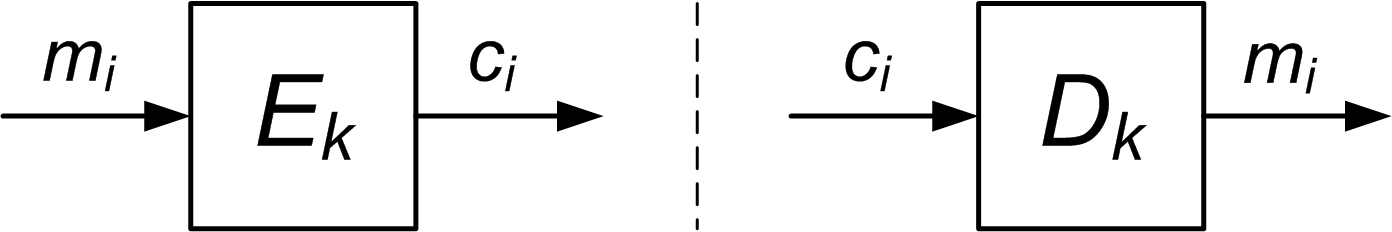
\includegraphics[width=.6\textwidth]{pict/blockcipher} }
            \mode<article>{ 
                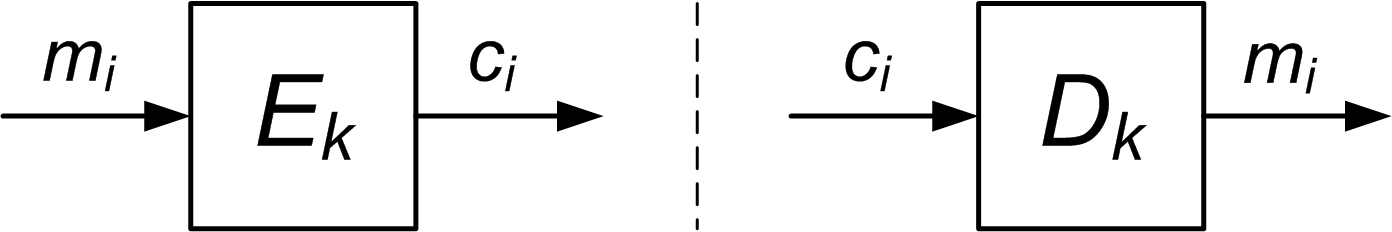
\includegraphics[width=.6\textwidth]{pict/blockcipher} 
                \caption{Блоки}\label{pict:blockcipher}
            }
        \end{center}
    \end{figure} 
    \mode<article>{См. рисунок \ref{pict:blockcipher}}
\end{frame}

Например, блоки можно уложить способом ECB, то есть без перекрытия и тогда кладка получится очень непрочной:

\begin{frame}
    \frametitle{ECB}
    
    \begin{figure}
        \begin{center}
            \mode<presentation>{ 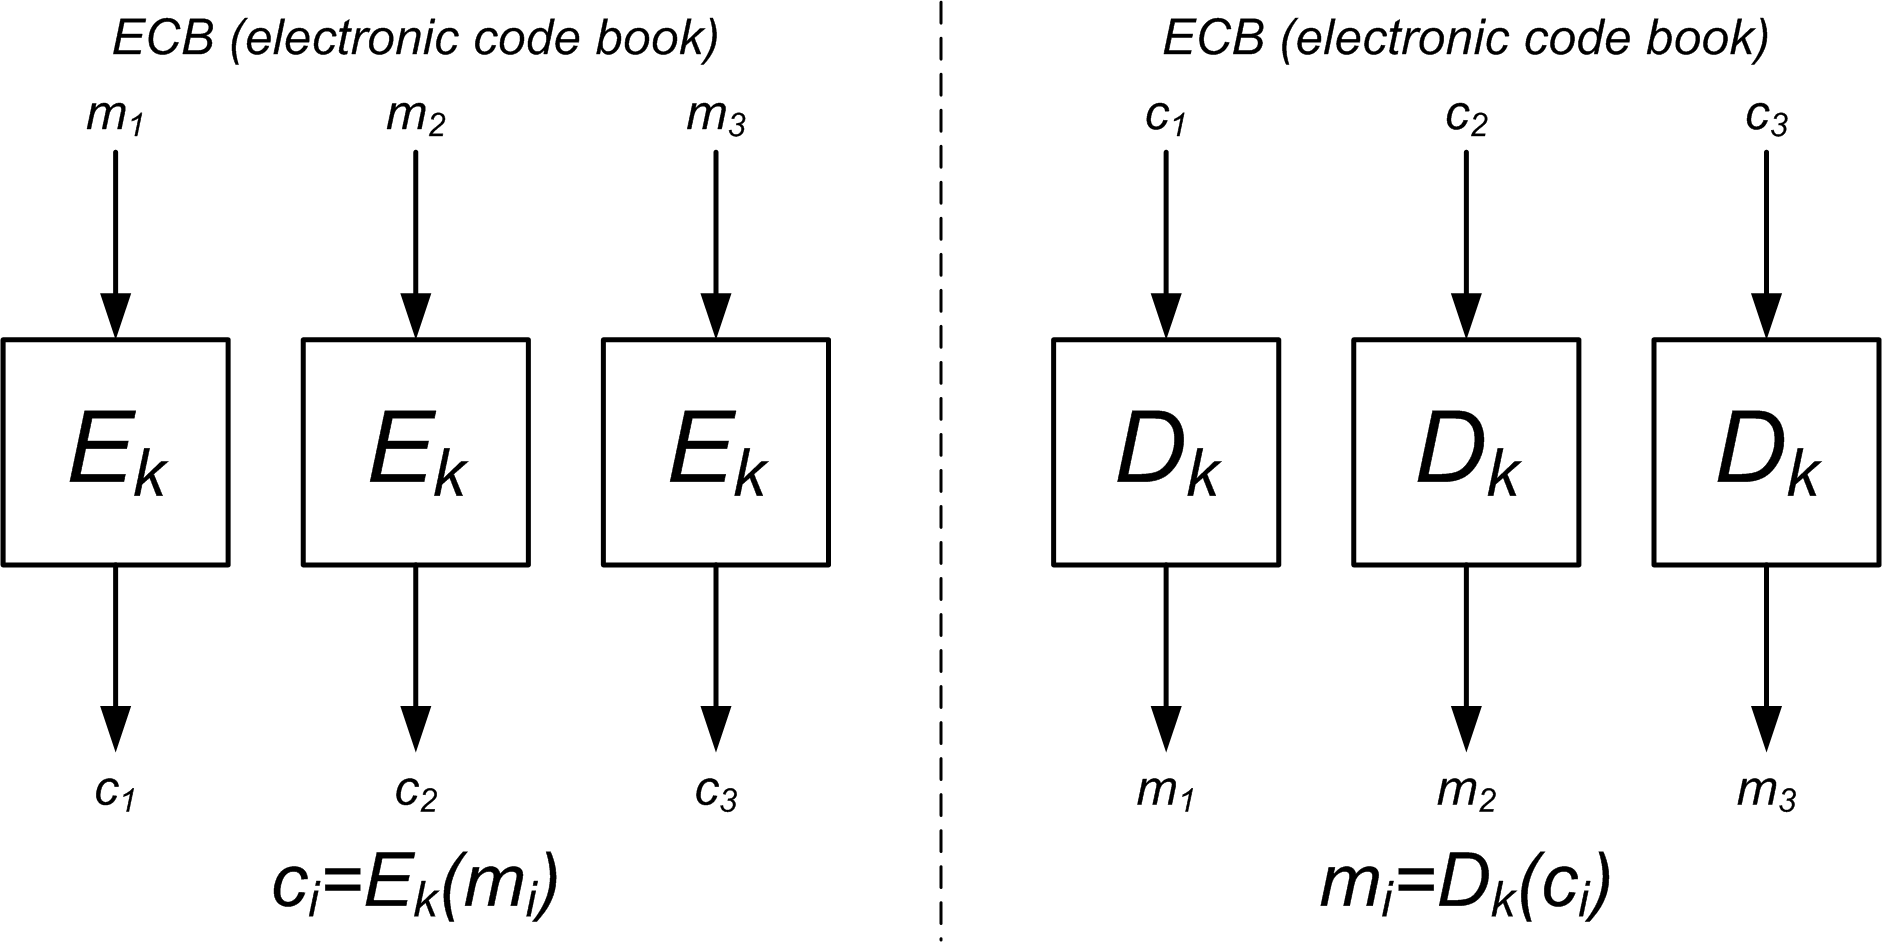
\includegraphics[width=.8\textwidth]{pict/ecb} }
            \mode<article>{ 
                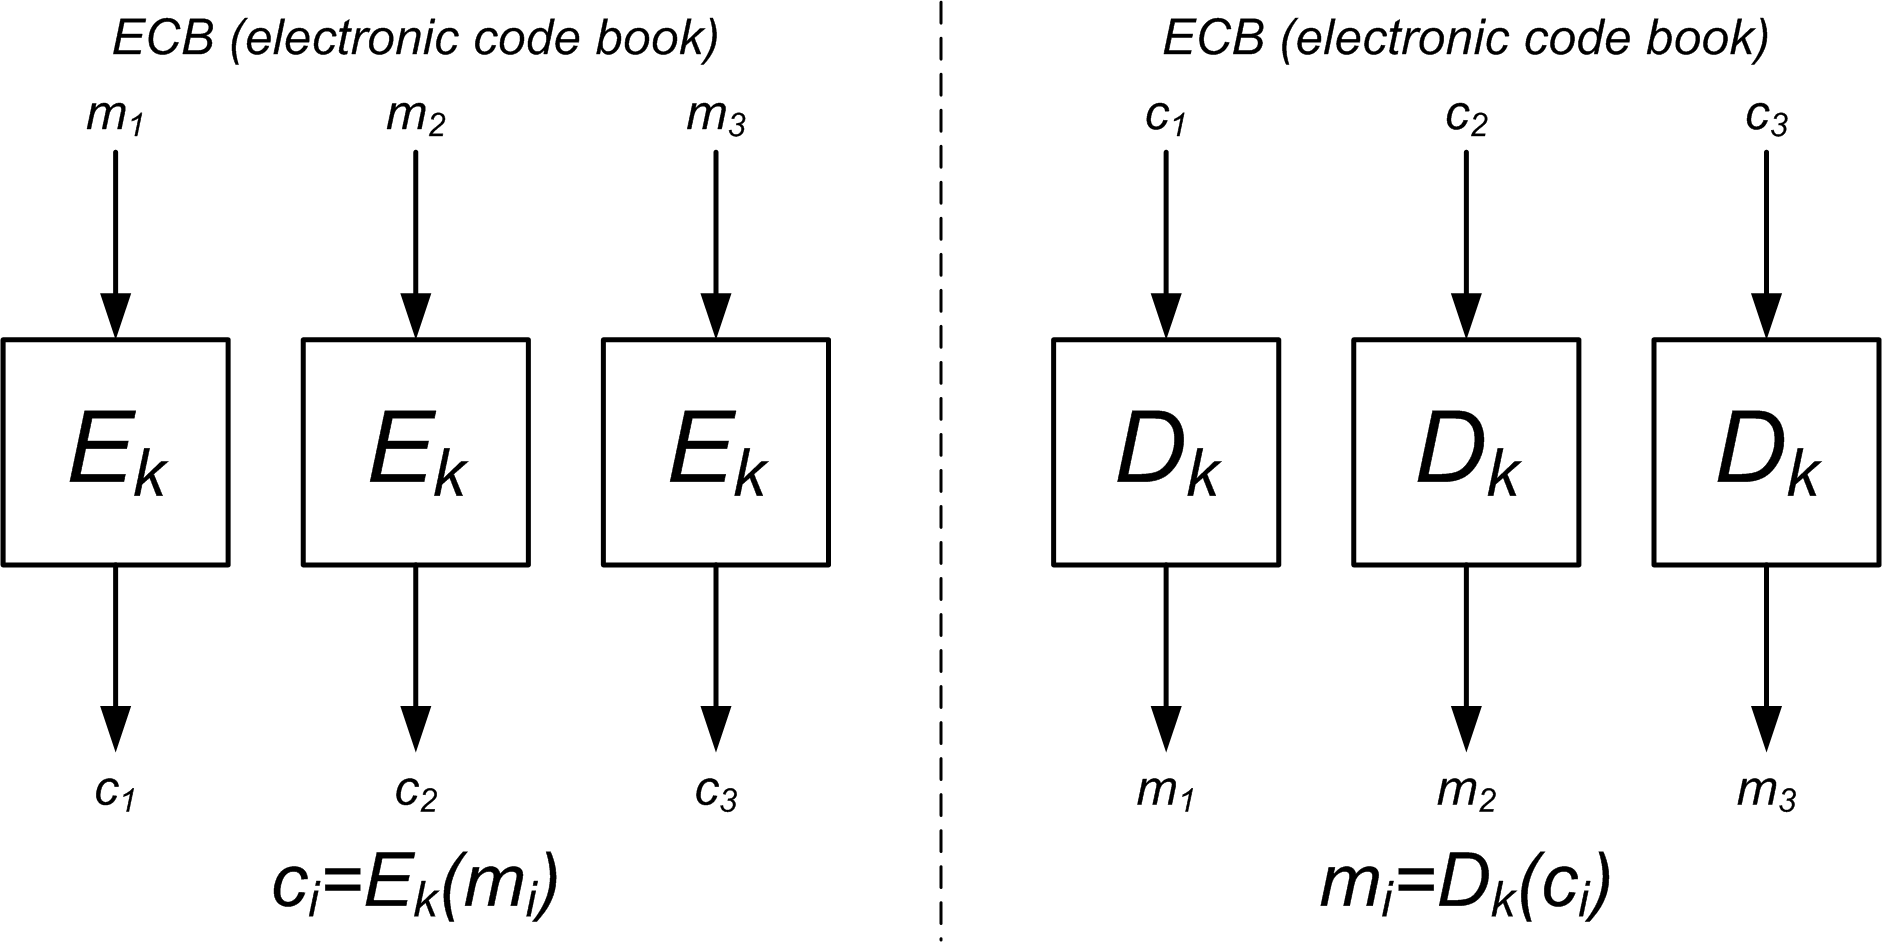
\includegraphics[width=.8\textwidth]{pict/ecb} 
                \caption{ECB}\label{pict:ecb}
            }
        \end{center}
    \end{figure} 
    \mode<article>{См. рисунок \ref{pict:ecb}}
\end{frame}


\begin{frame}
    \frametitle{ECB}
    
    \begin{figure}
        \begin{center}
            \mode<presentation>{ 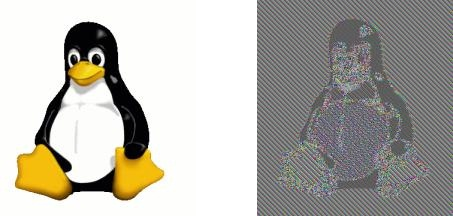
\includegraphics[width=.8\textwidth]{pict/tuxEcb} }
            \mode<article>{ 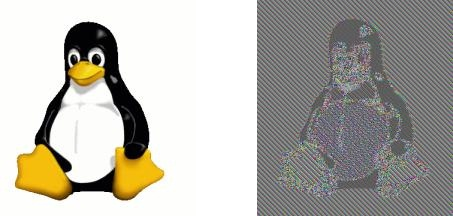
\includegraphics[width=.8\textwidth]{pict/tuxEcb} }
        \end{center}
        \caption{Изображение Tux\footnote{\copyright Larry Ewing. lewing@isc.tamu.edu} зашифровано в режиме ECB\footnote{Заимствовано из http://en.wikipedia.org/wiki/Image:Tux\_ecb.jpg}.}\label{pict:tuxEcb}
    \end{figure} 
    \mode<article>{См. рисунок \ref{pict:tuxEcb}}
\end{frame}


\begin{frame}
    \frametitle{No ECB}
    
    \begin{figure}
        \begin{center}
            \mode<presentation>{ 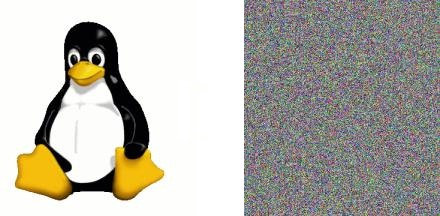
\includegraphics[width=.8\textwidth]{pict/tuxSecure} }
            \mode<article>{ 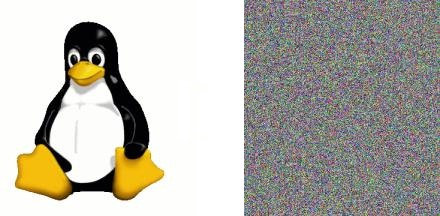
\includegraphics[width=.8\textwidth]{pict/tuxSecure} }
        \end{center}
        \caption{Изображение Tux\footnote{\copyright Larry Ewing. lewing@isc.tamu.edu} зашифровано в режиме, отличном от ECB\footnote{Заимствовано из http://en.wikipedia.org/wiki/Image:Tux\_secure.jpg}.}\label{pict:tuxSecure}
    \end{figure} 
    \mode<article>{См. рисунок \ref{pict:tuxSecure}}
\end{frame}

Недостатки очевидны (даже из рисунка пингвинёнка\ref{pict:tuxEcb} (заимствован из википедии\ldots)). Подмена одного из блоков в канале не скажется на дешифровании остальных блоков (отчасти это и достоинство – большая устойчивость к ошибкам). Также недостатком считается атаки с удалениями и вставками, например, выражение <<Плати Алисе сто фунтов не плати бобу двести фунтов>>, в котором каждому слову соответствует блок, после шифрования будет соответствовать, также пословно, выражение <<У кошки четыре ноги а у человека две ноги>>.  При возможности активного перехвата можно послать сообщения:

<<а У кошки четыре ноги у человека две ноги>>,
<<У кошки две ноги а у человека четыре ноги>>,
<<У кошки две ноги у человека две ноги>>.

Которые дадут весьма неприятный результат. Бороться с этим можно добавляя служебную информацию в каждый блок (например, контрольные суммы предыдущих блоков, или номер блока).

Достоинство – очевидный способ распараллеливания и как следствие – это самый быстрый режим шифрования.

Можно уложить методом CBC, тогда блоки уже не будут взаимонезависимыми

\begin{frame}
    \frametitle{CBC}
    
    \begin{figure}
        \begin{center}
            \mode<presentation>{ 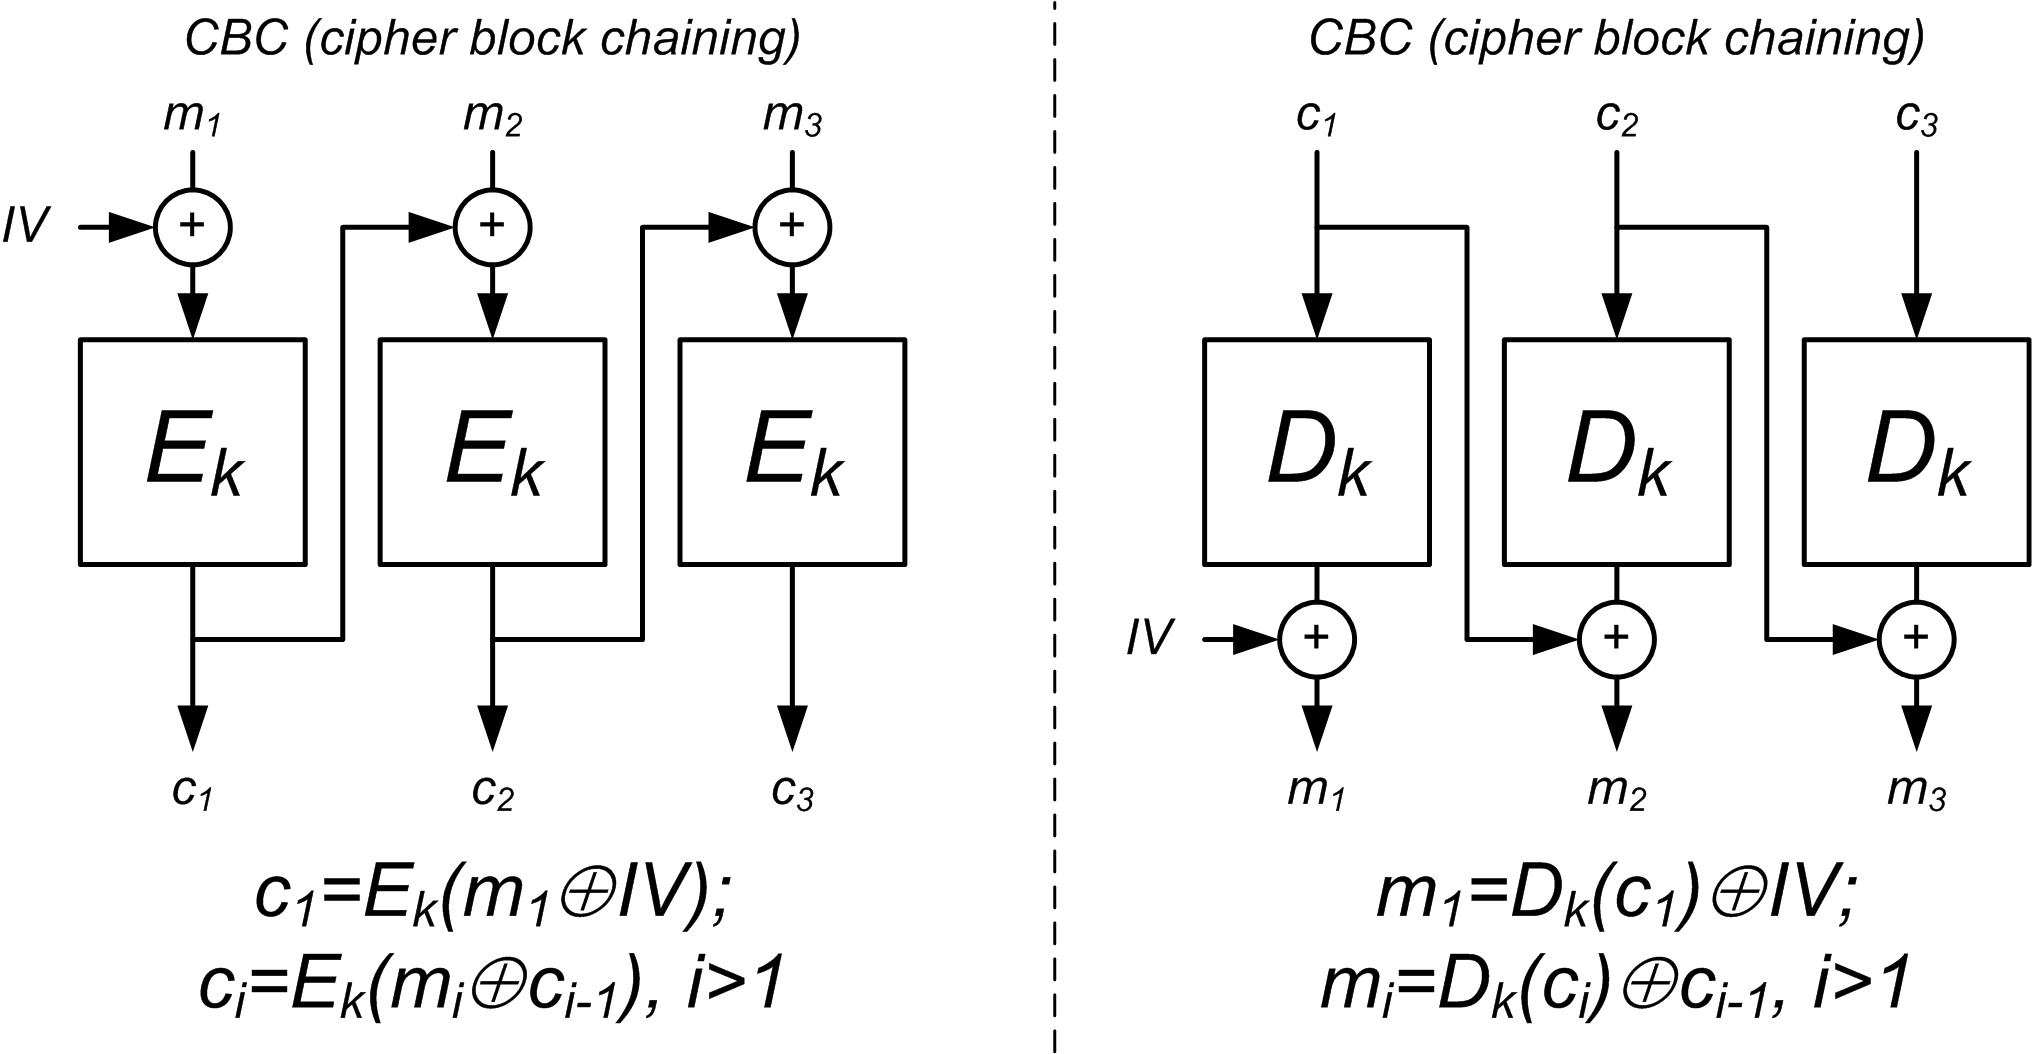
\includegraphics[width=.8\textwidth]{pict/cbc} }
            \mode<article>{ 
                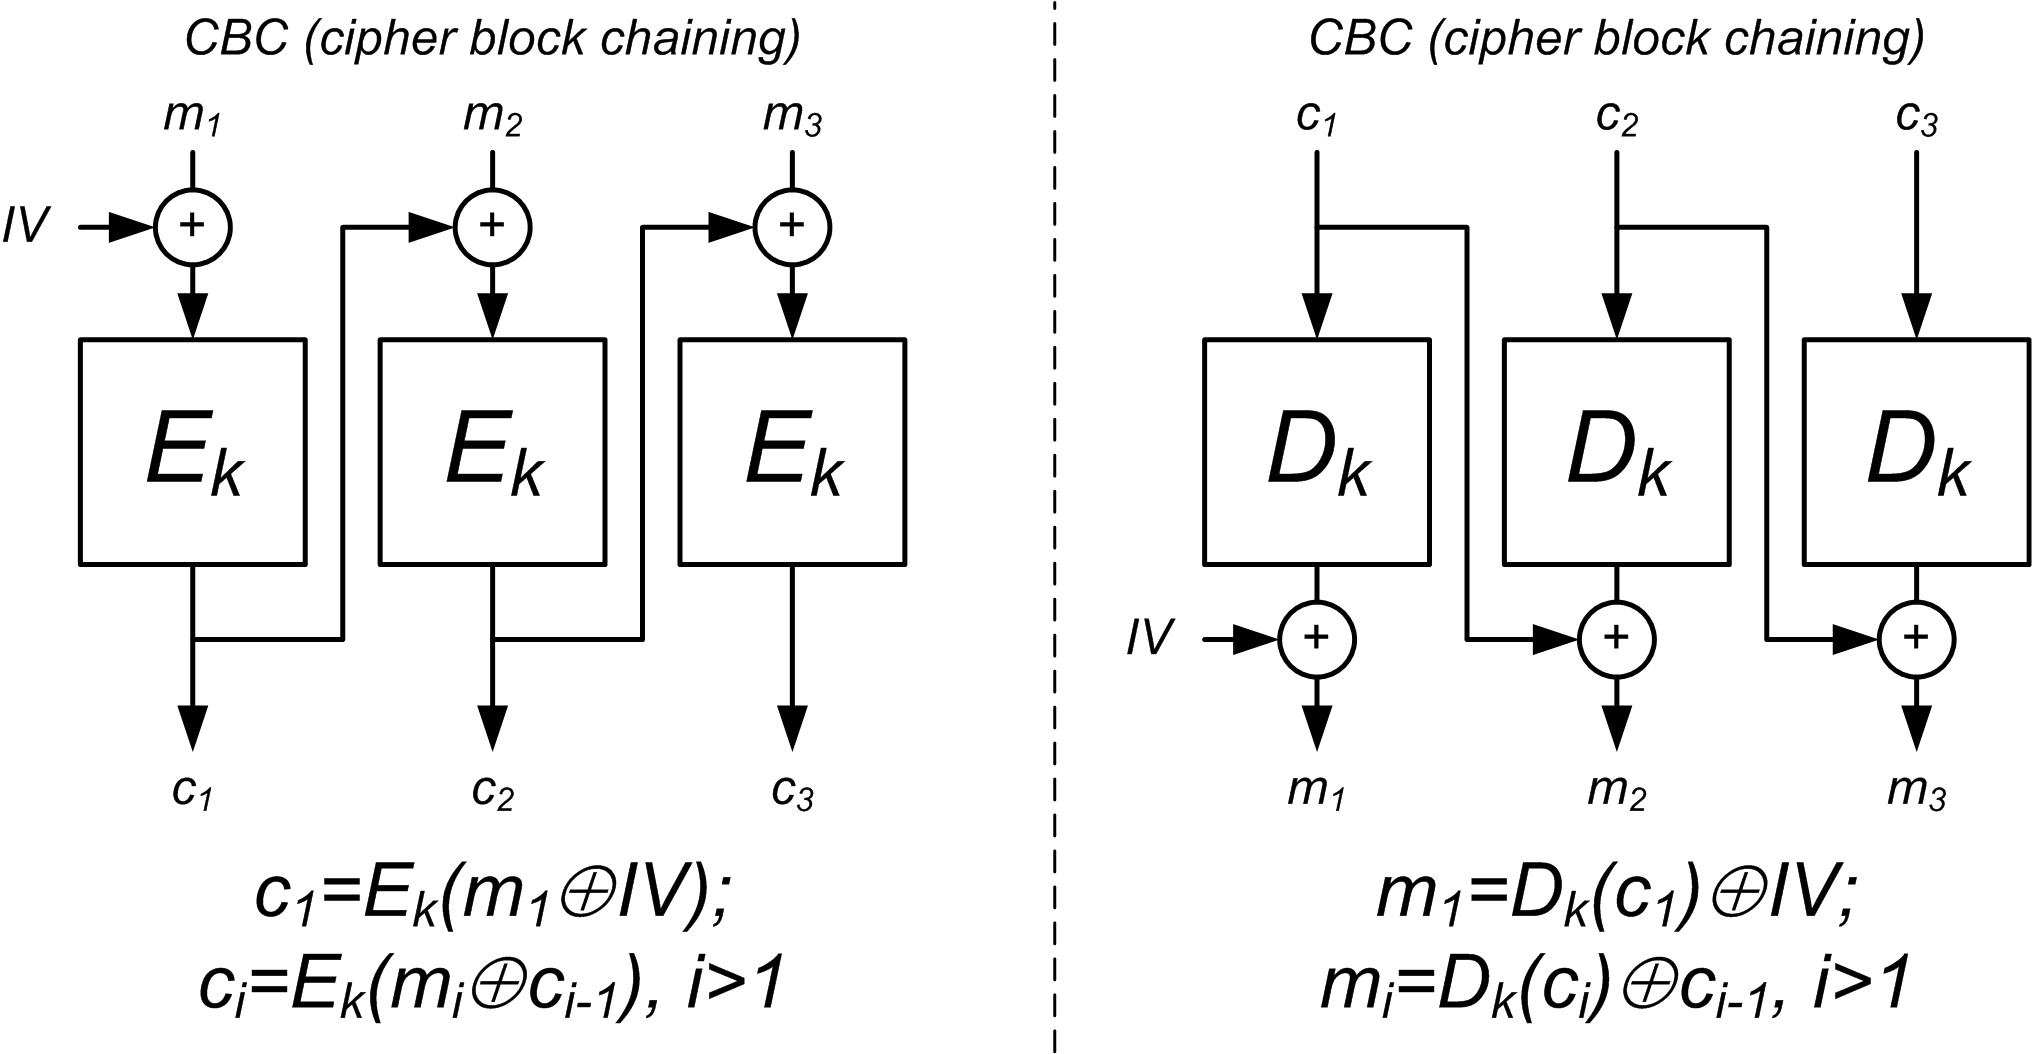
\includegraphics[width=.8\textwidth]{pict/cbc} 
                \caption{CBC}\label{pict:cbc}
            }
        \end{center}
    \end{figure} 
    \mode<article>{См. рисунок \ref{pict:cbc}}
\end{frame}

Считается наилучшим способом эксплуатации блочного шифра, поскольку предназначен для предотвращения потерь с использованием удалений и вставок.

\begin{frame}
    \frametitle{CFB}
    \framesubtitle{Общий случай}
    
    \begin{figure}
        \begin{center}
            \mode<presentation>{ 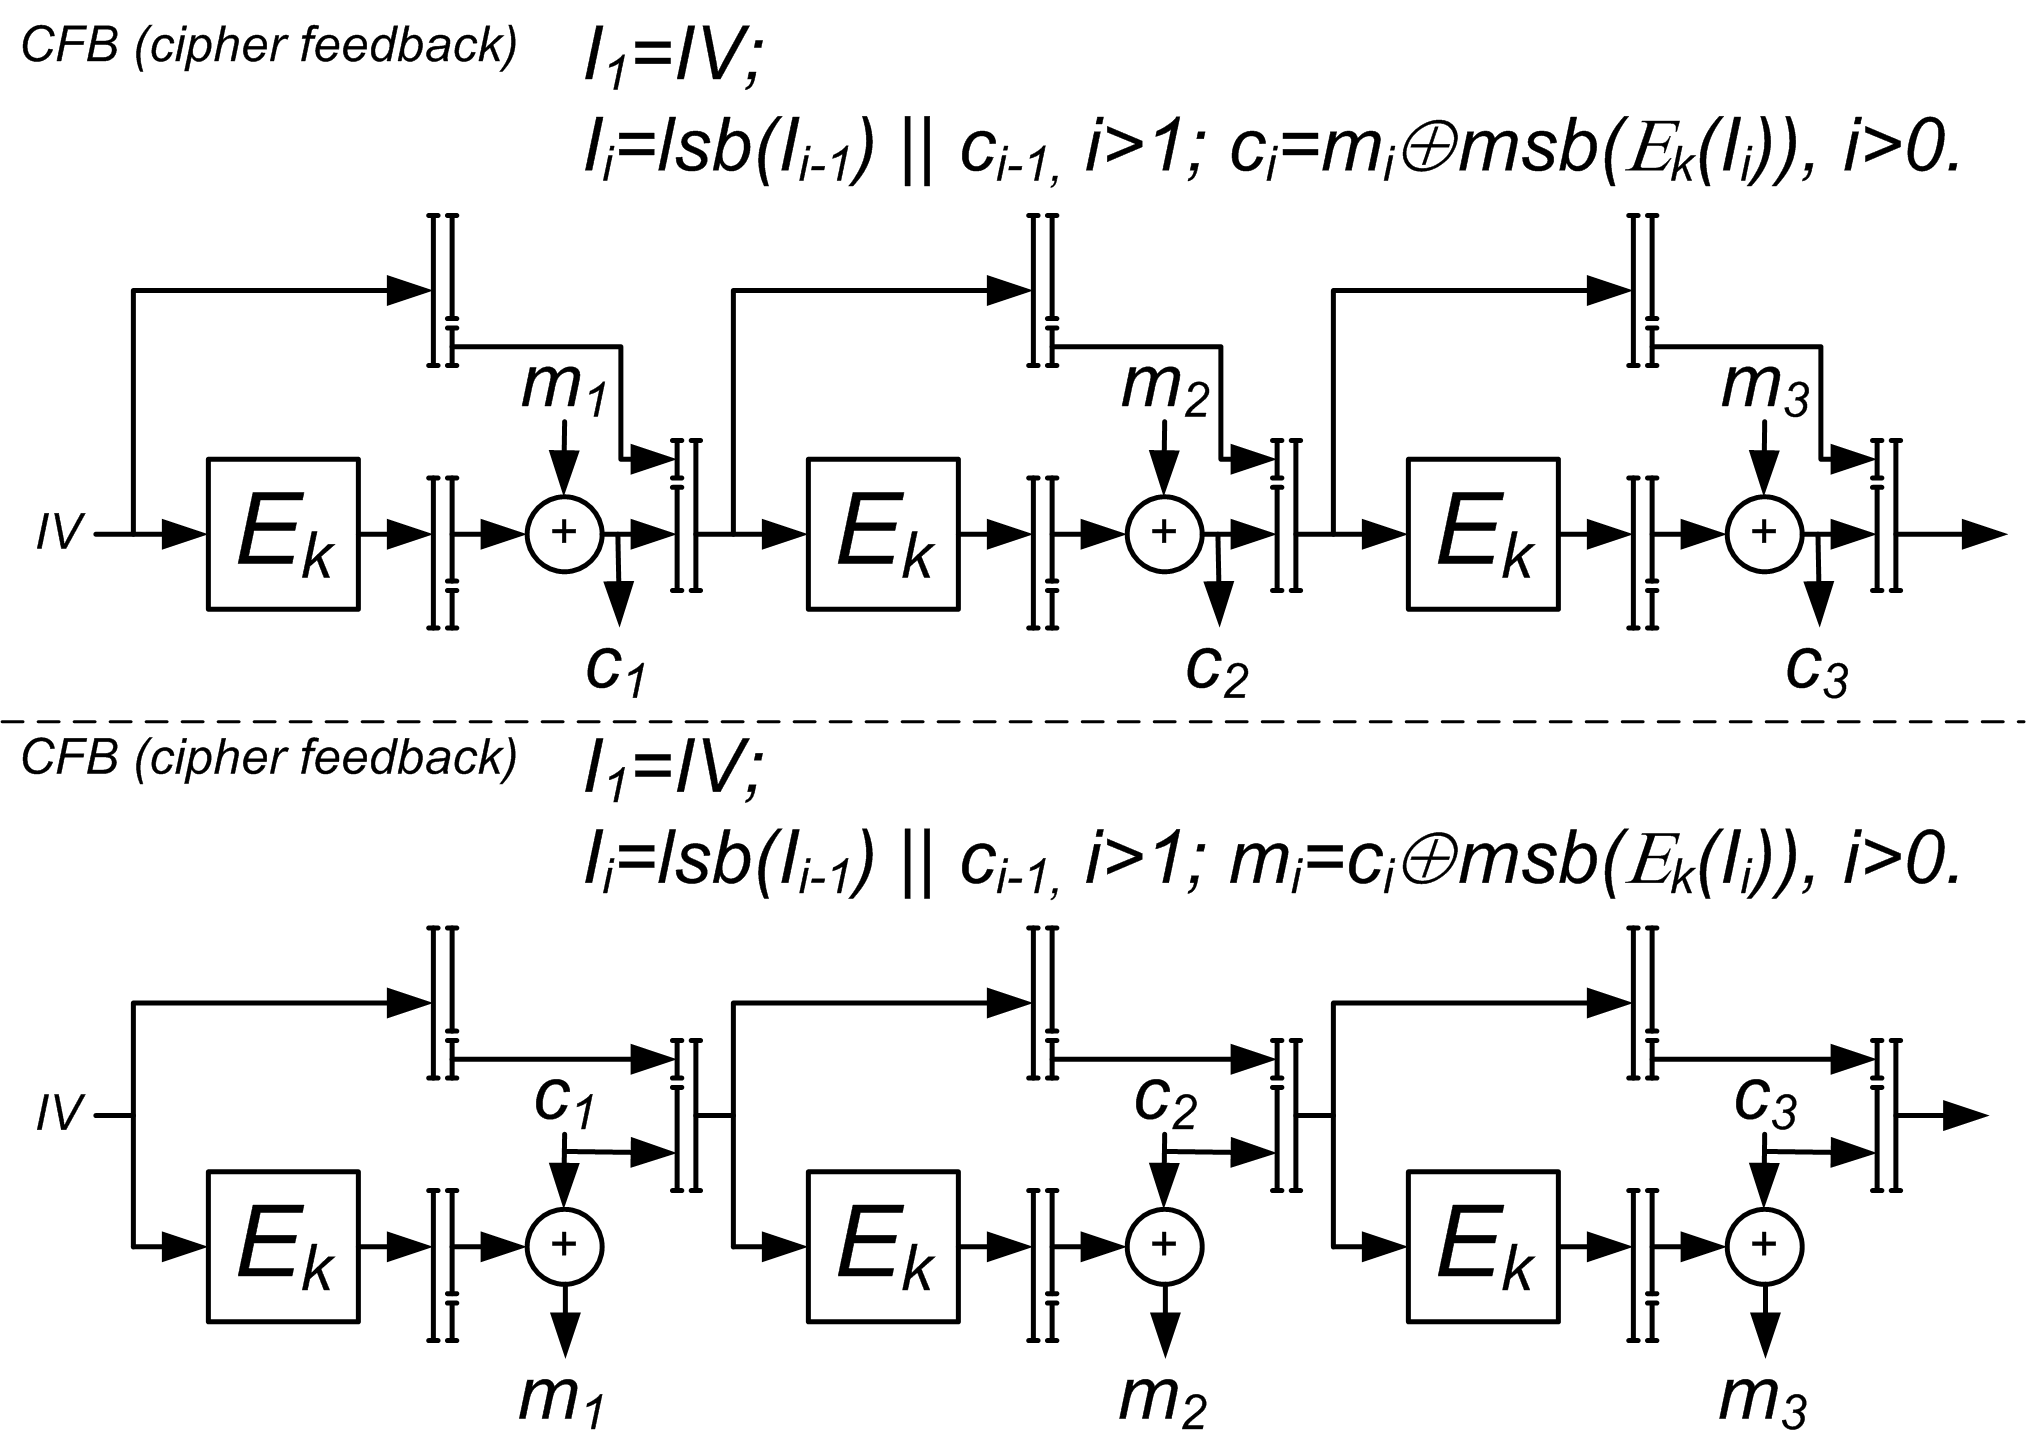
\includegraphics[height=.7\textheight]{pict/cfb2} }
            \mode<article>{ 
                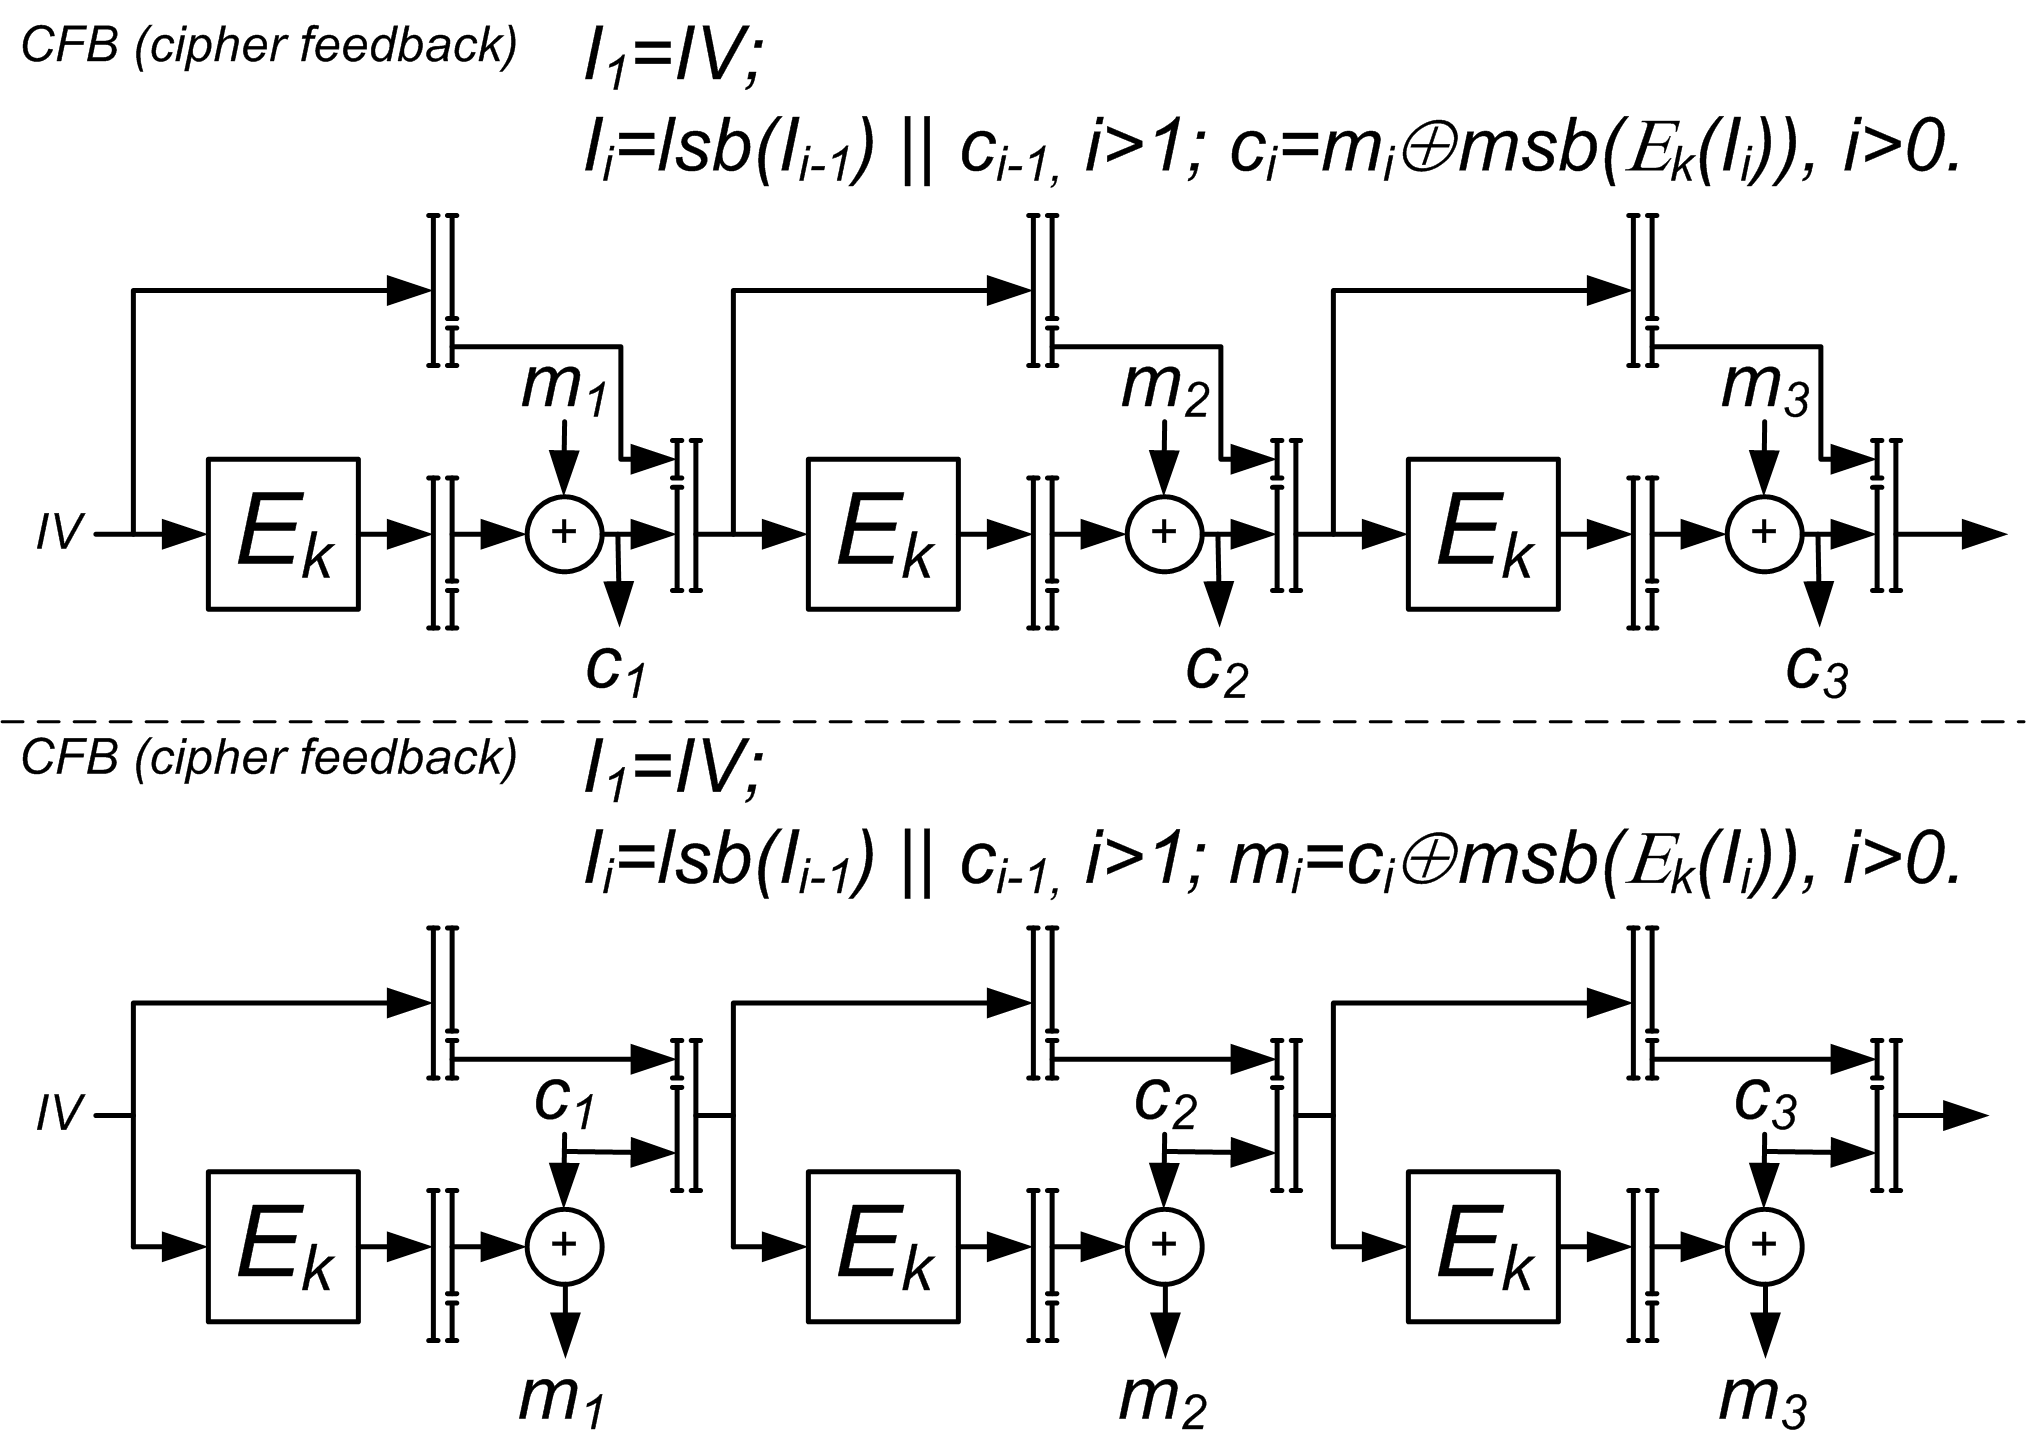
\includegraphics[width=.8\textwidth]{pict/cfb2} 
                \caption{CFB}\label{pict:cfb2}
            }
        \end{center}
    \end{figure} 
    \mode<article>{См. рисунок \ref{pict:cfb2}}
    $X=msb(X)||lsb(X)$. $msb(x)$ --- $s$ старших бит, а $lsb(x)$ --- $n-s$ младших. $s$ --- размер блока. 
\end{frame}


\begin{frame}
    \frametitle{CFB}
    \framesubtitle{Частный случай}

    \begin{figure}
        \begin{center}
            \mode<presentation>{ 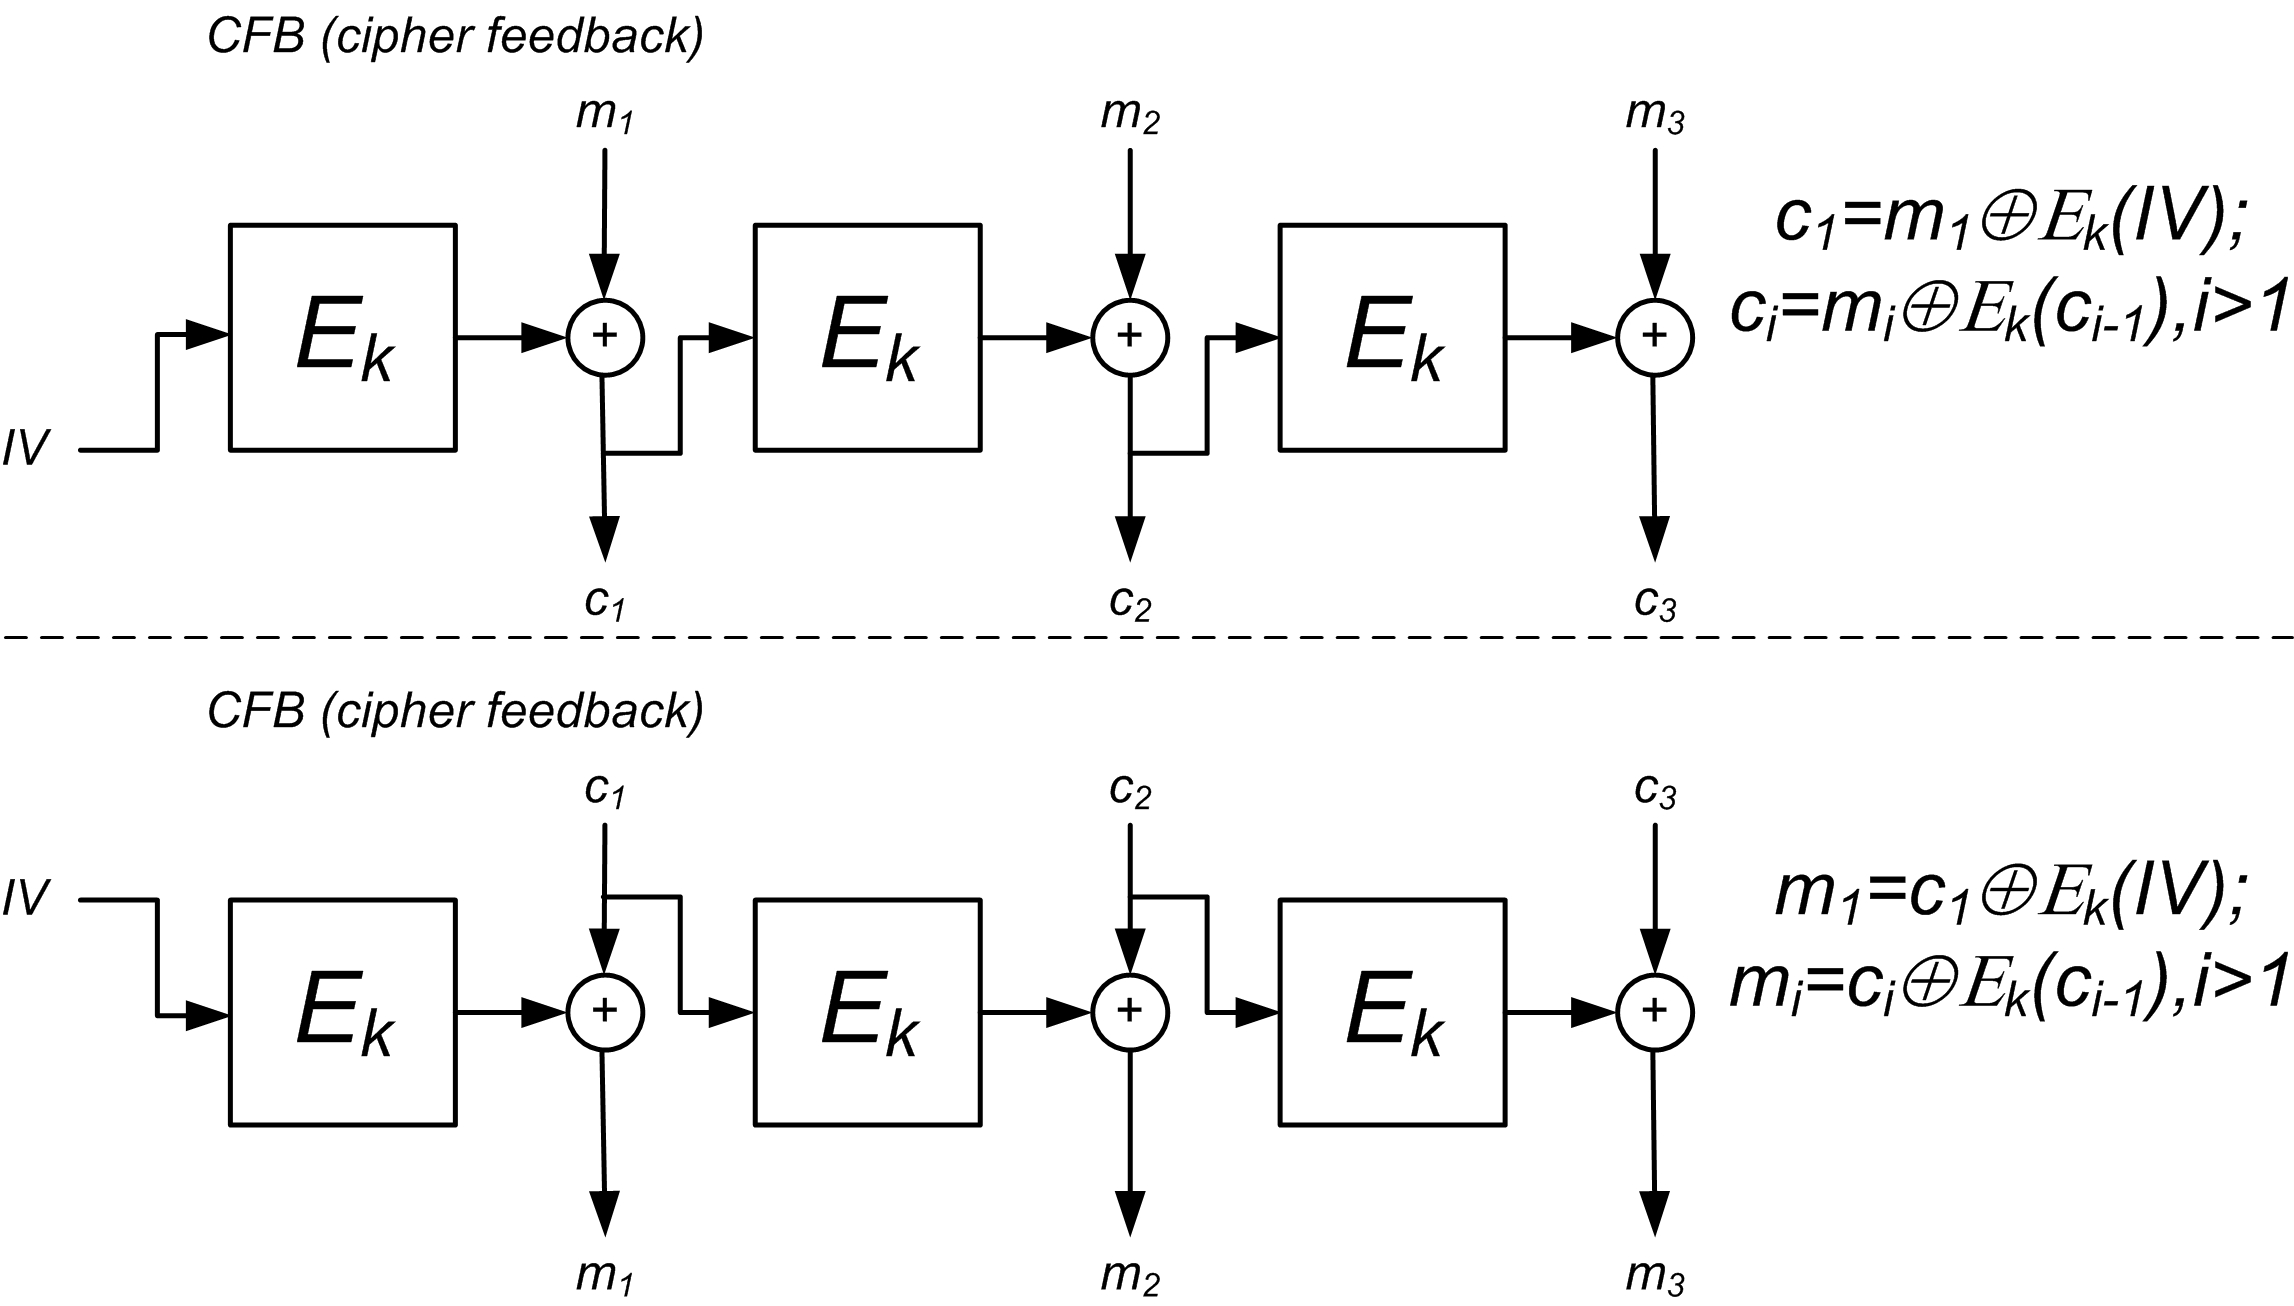
\includegraphics[width=.8\textwidth]{pict/cfb} }
            \mode<article>{ 
                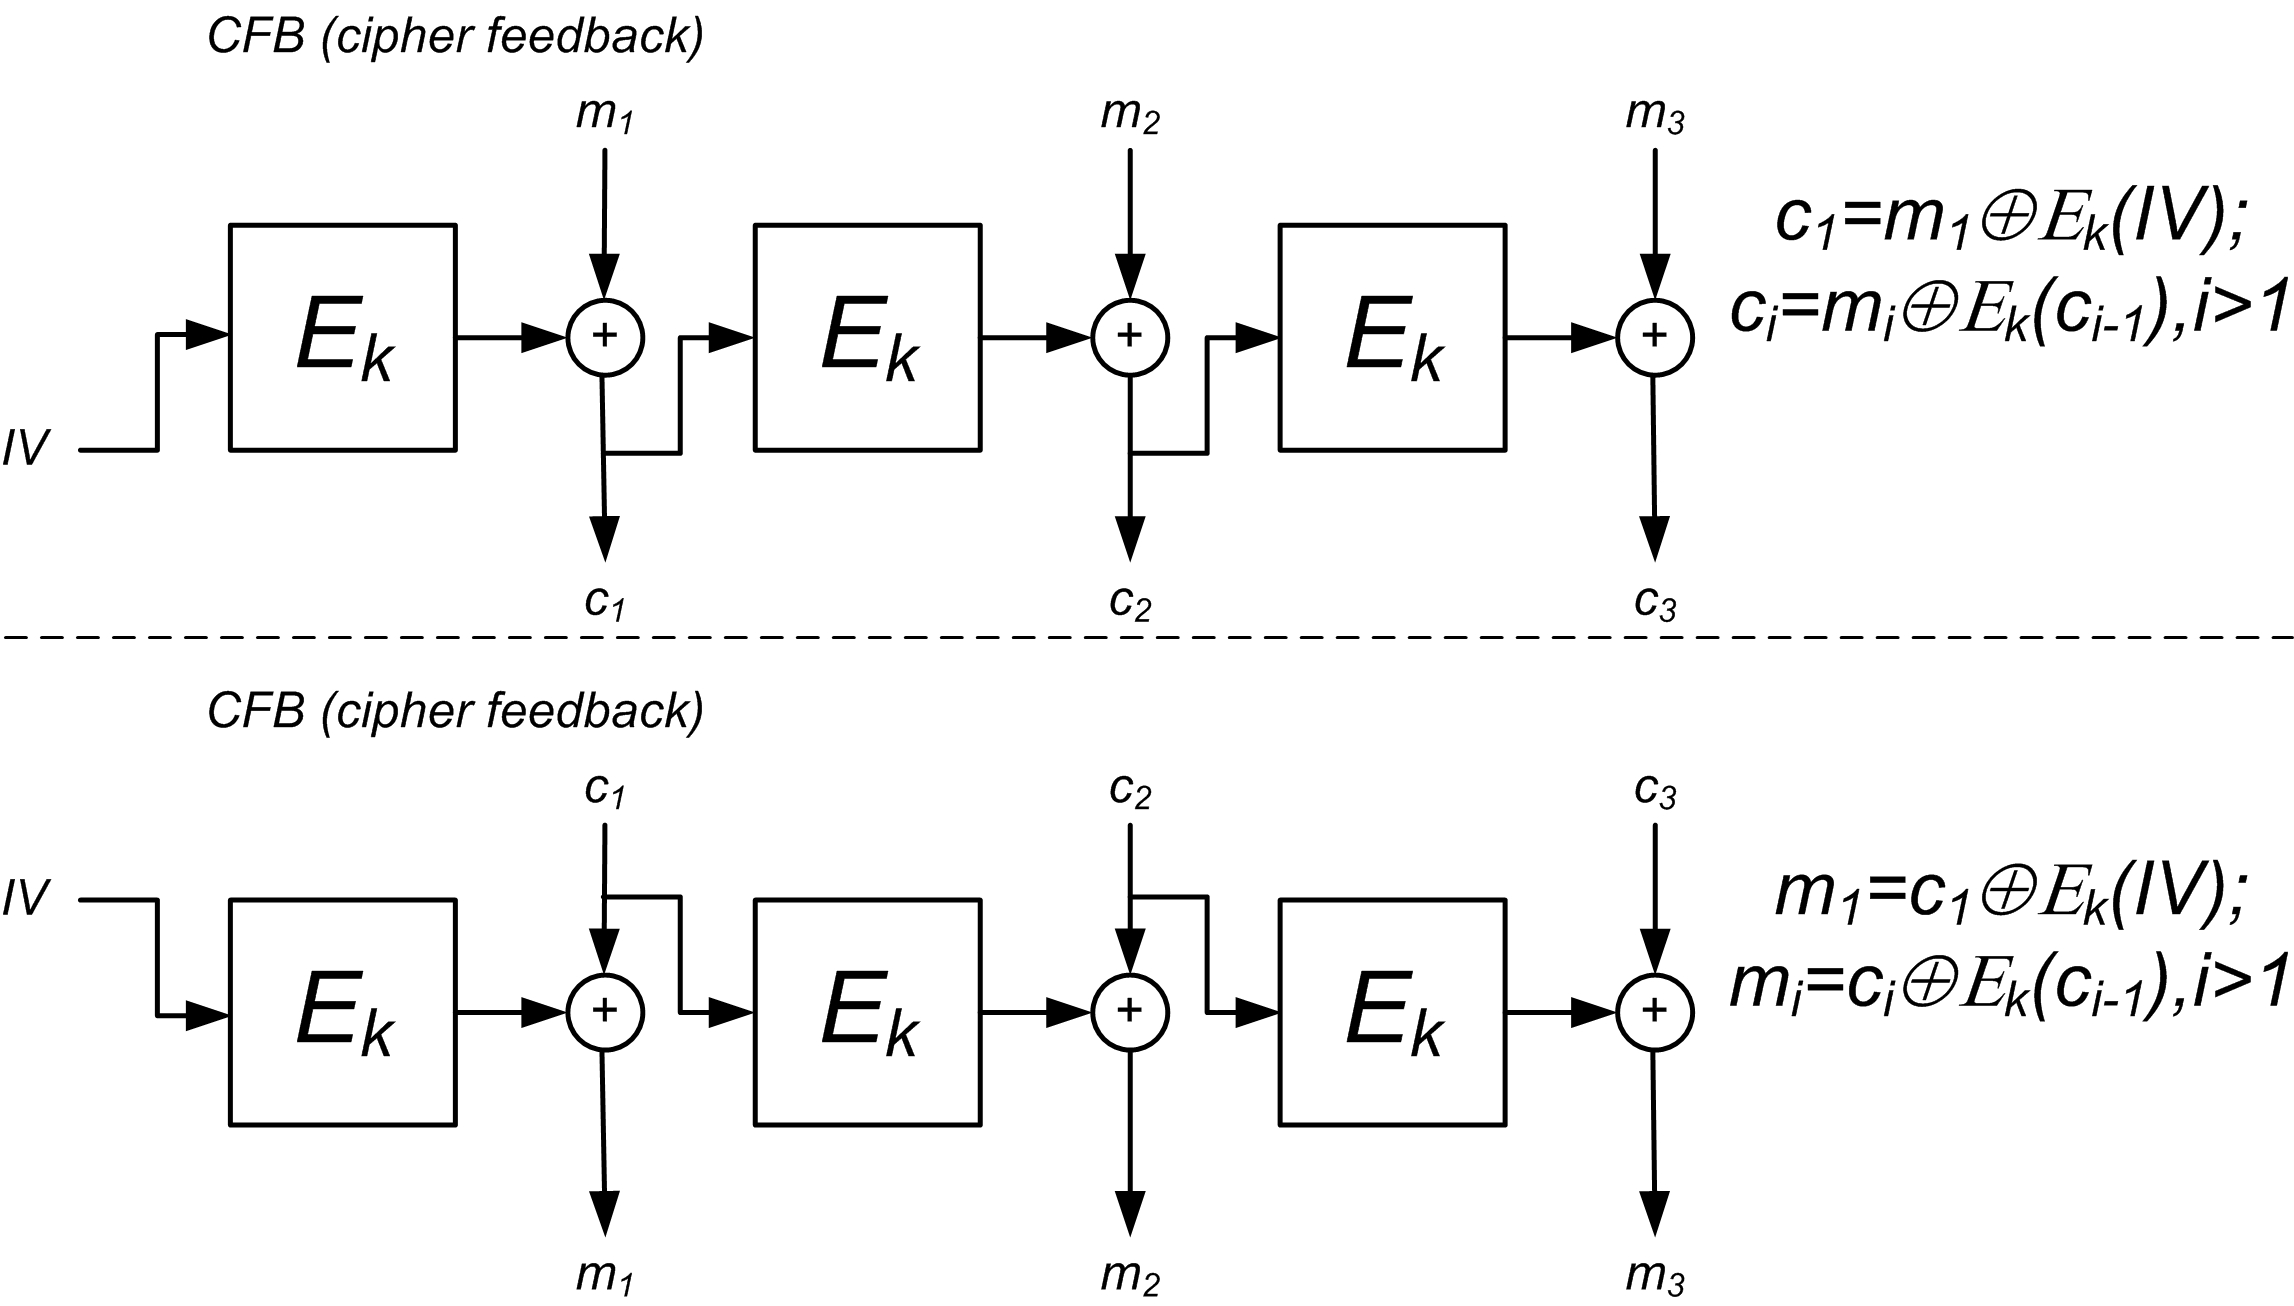
\includegraphics[width=.8\textwidth]{pict/cfb} 
                \caption{CFB}\label{pict:cfb}
            }
        \end{center}
    \end{figure} 
    \mode<article>{См. рисунок \ref{pict:cfb}}
\end{frame}


\begin{frame}
    \frametitle{OFB}
    
    \begin{figure}
        \begin{center}
            \mode<presentation>{ 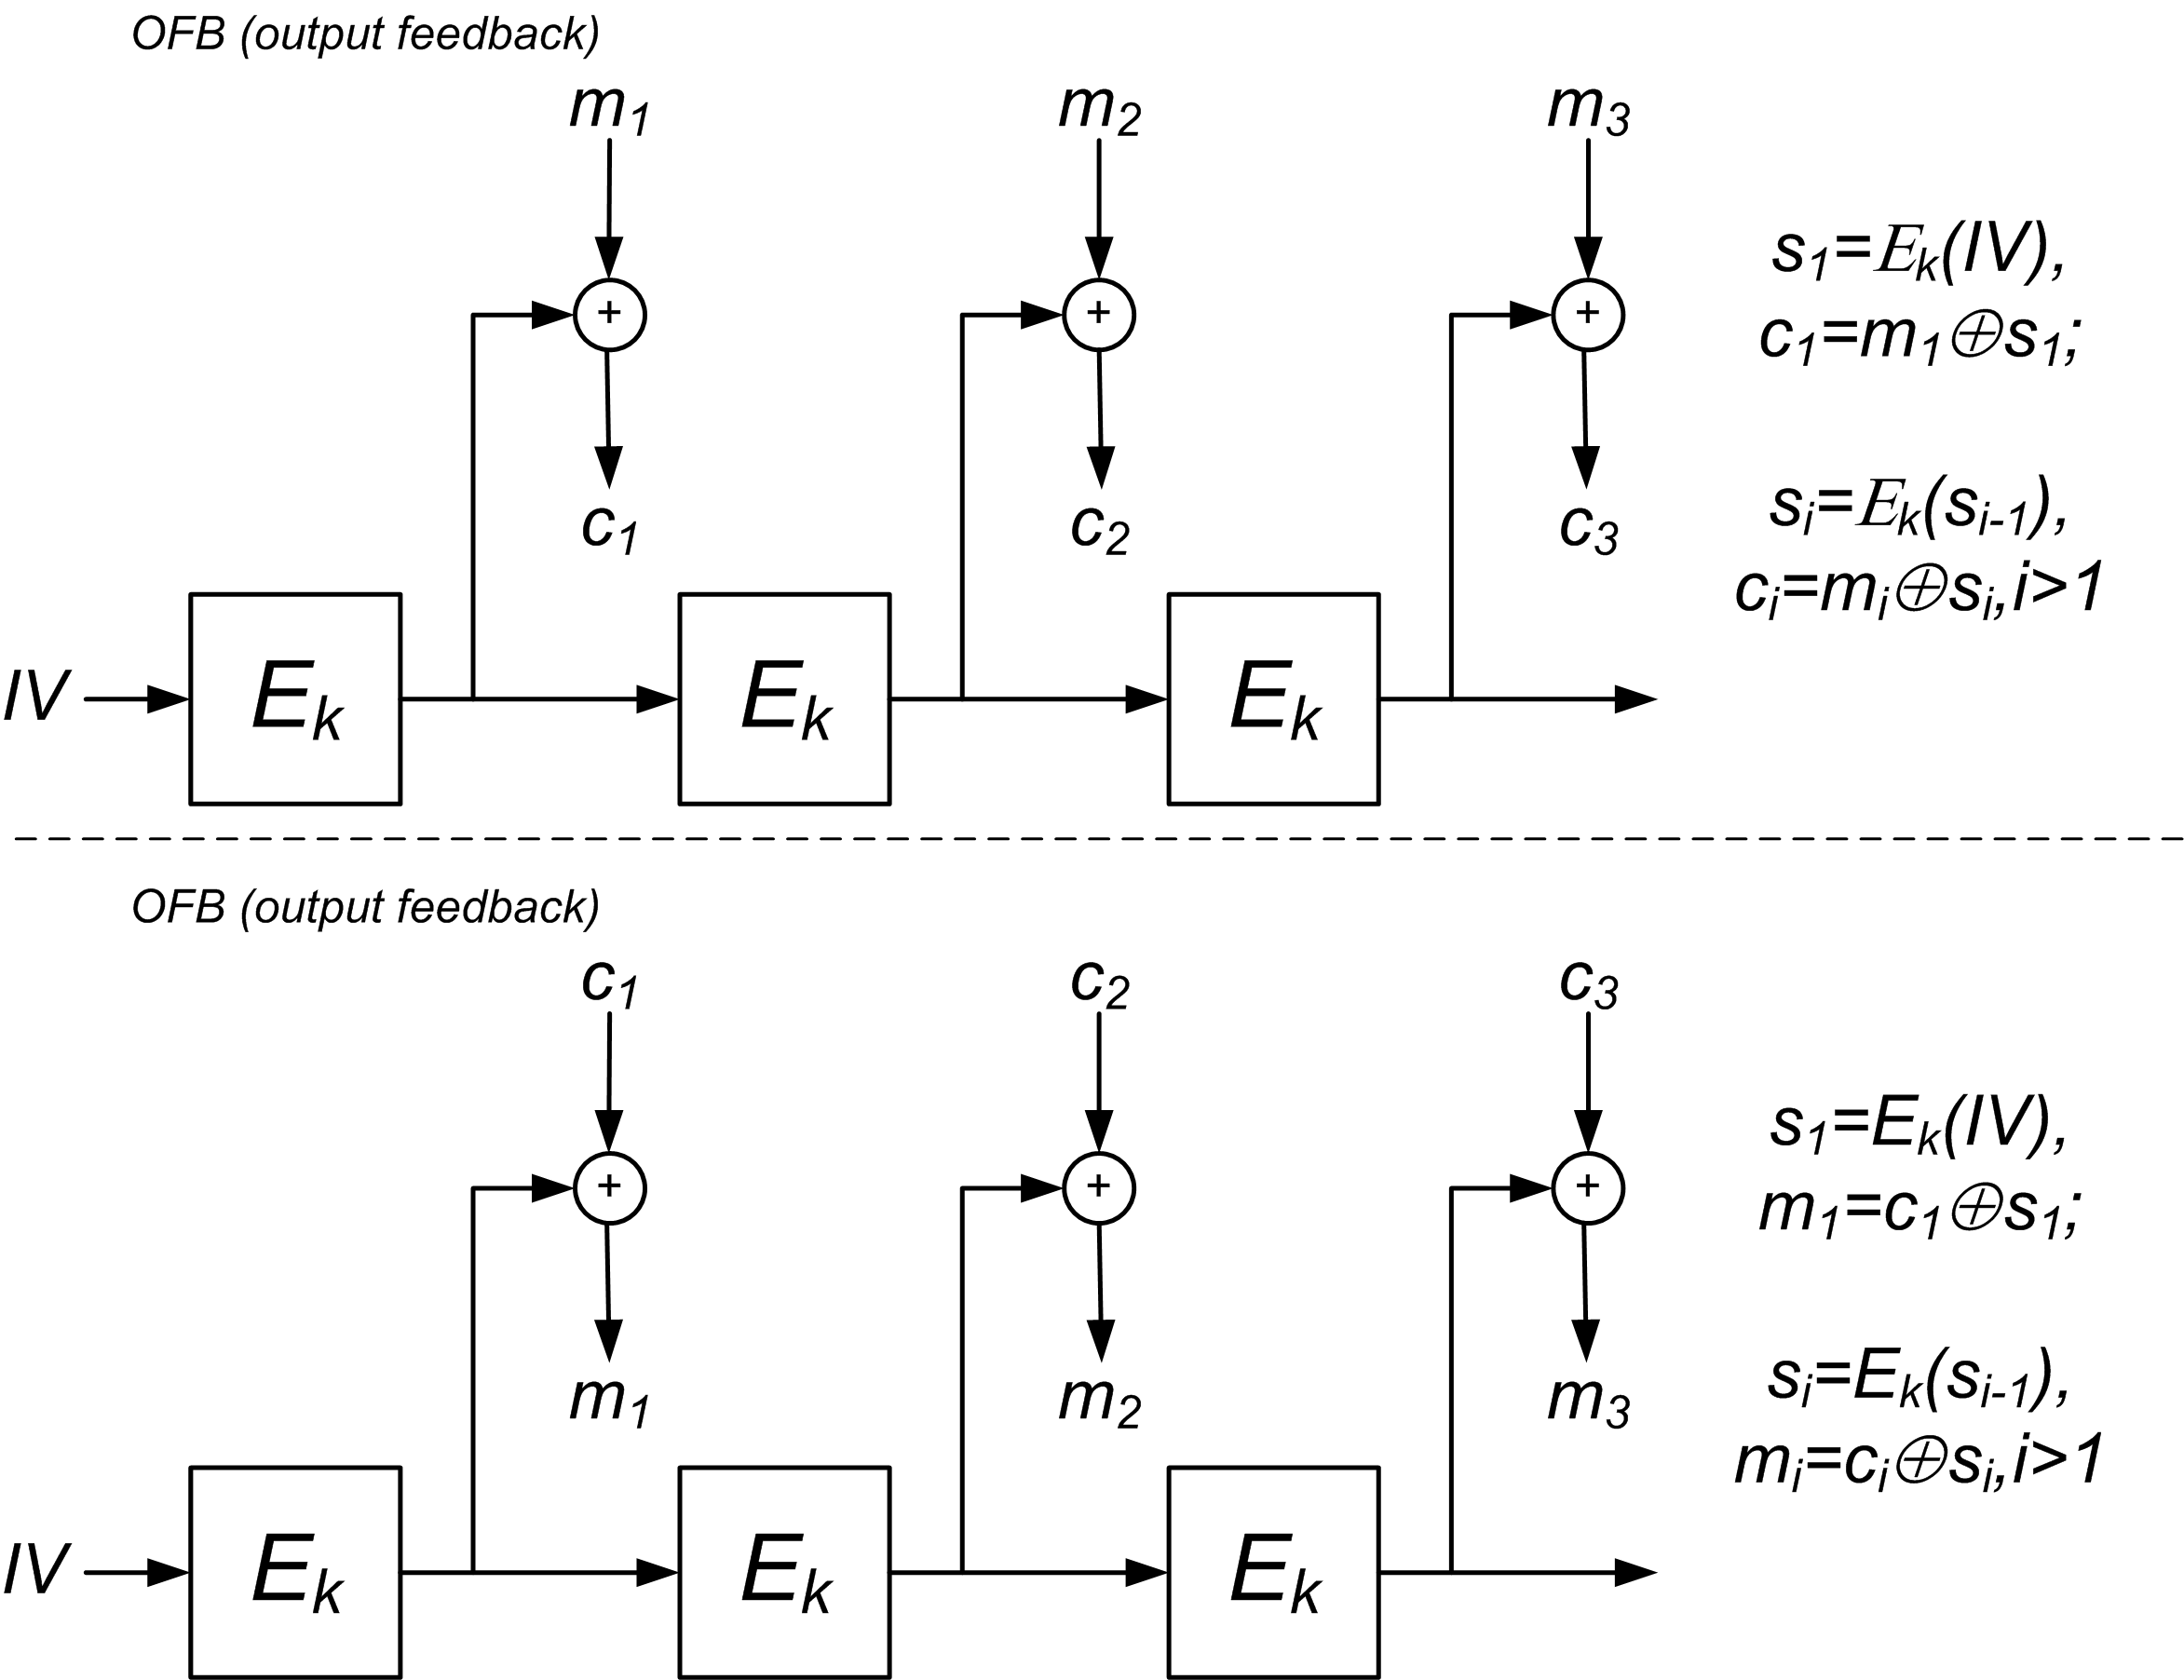
\includegraphics[height=.73\textheight]{pict/ofb} }
            \mode<article>{ 
                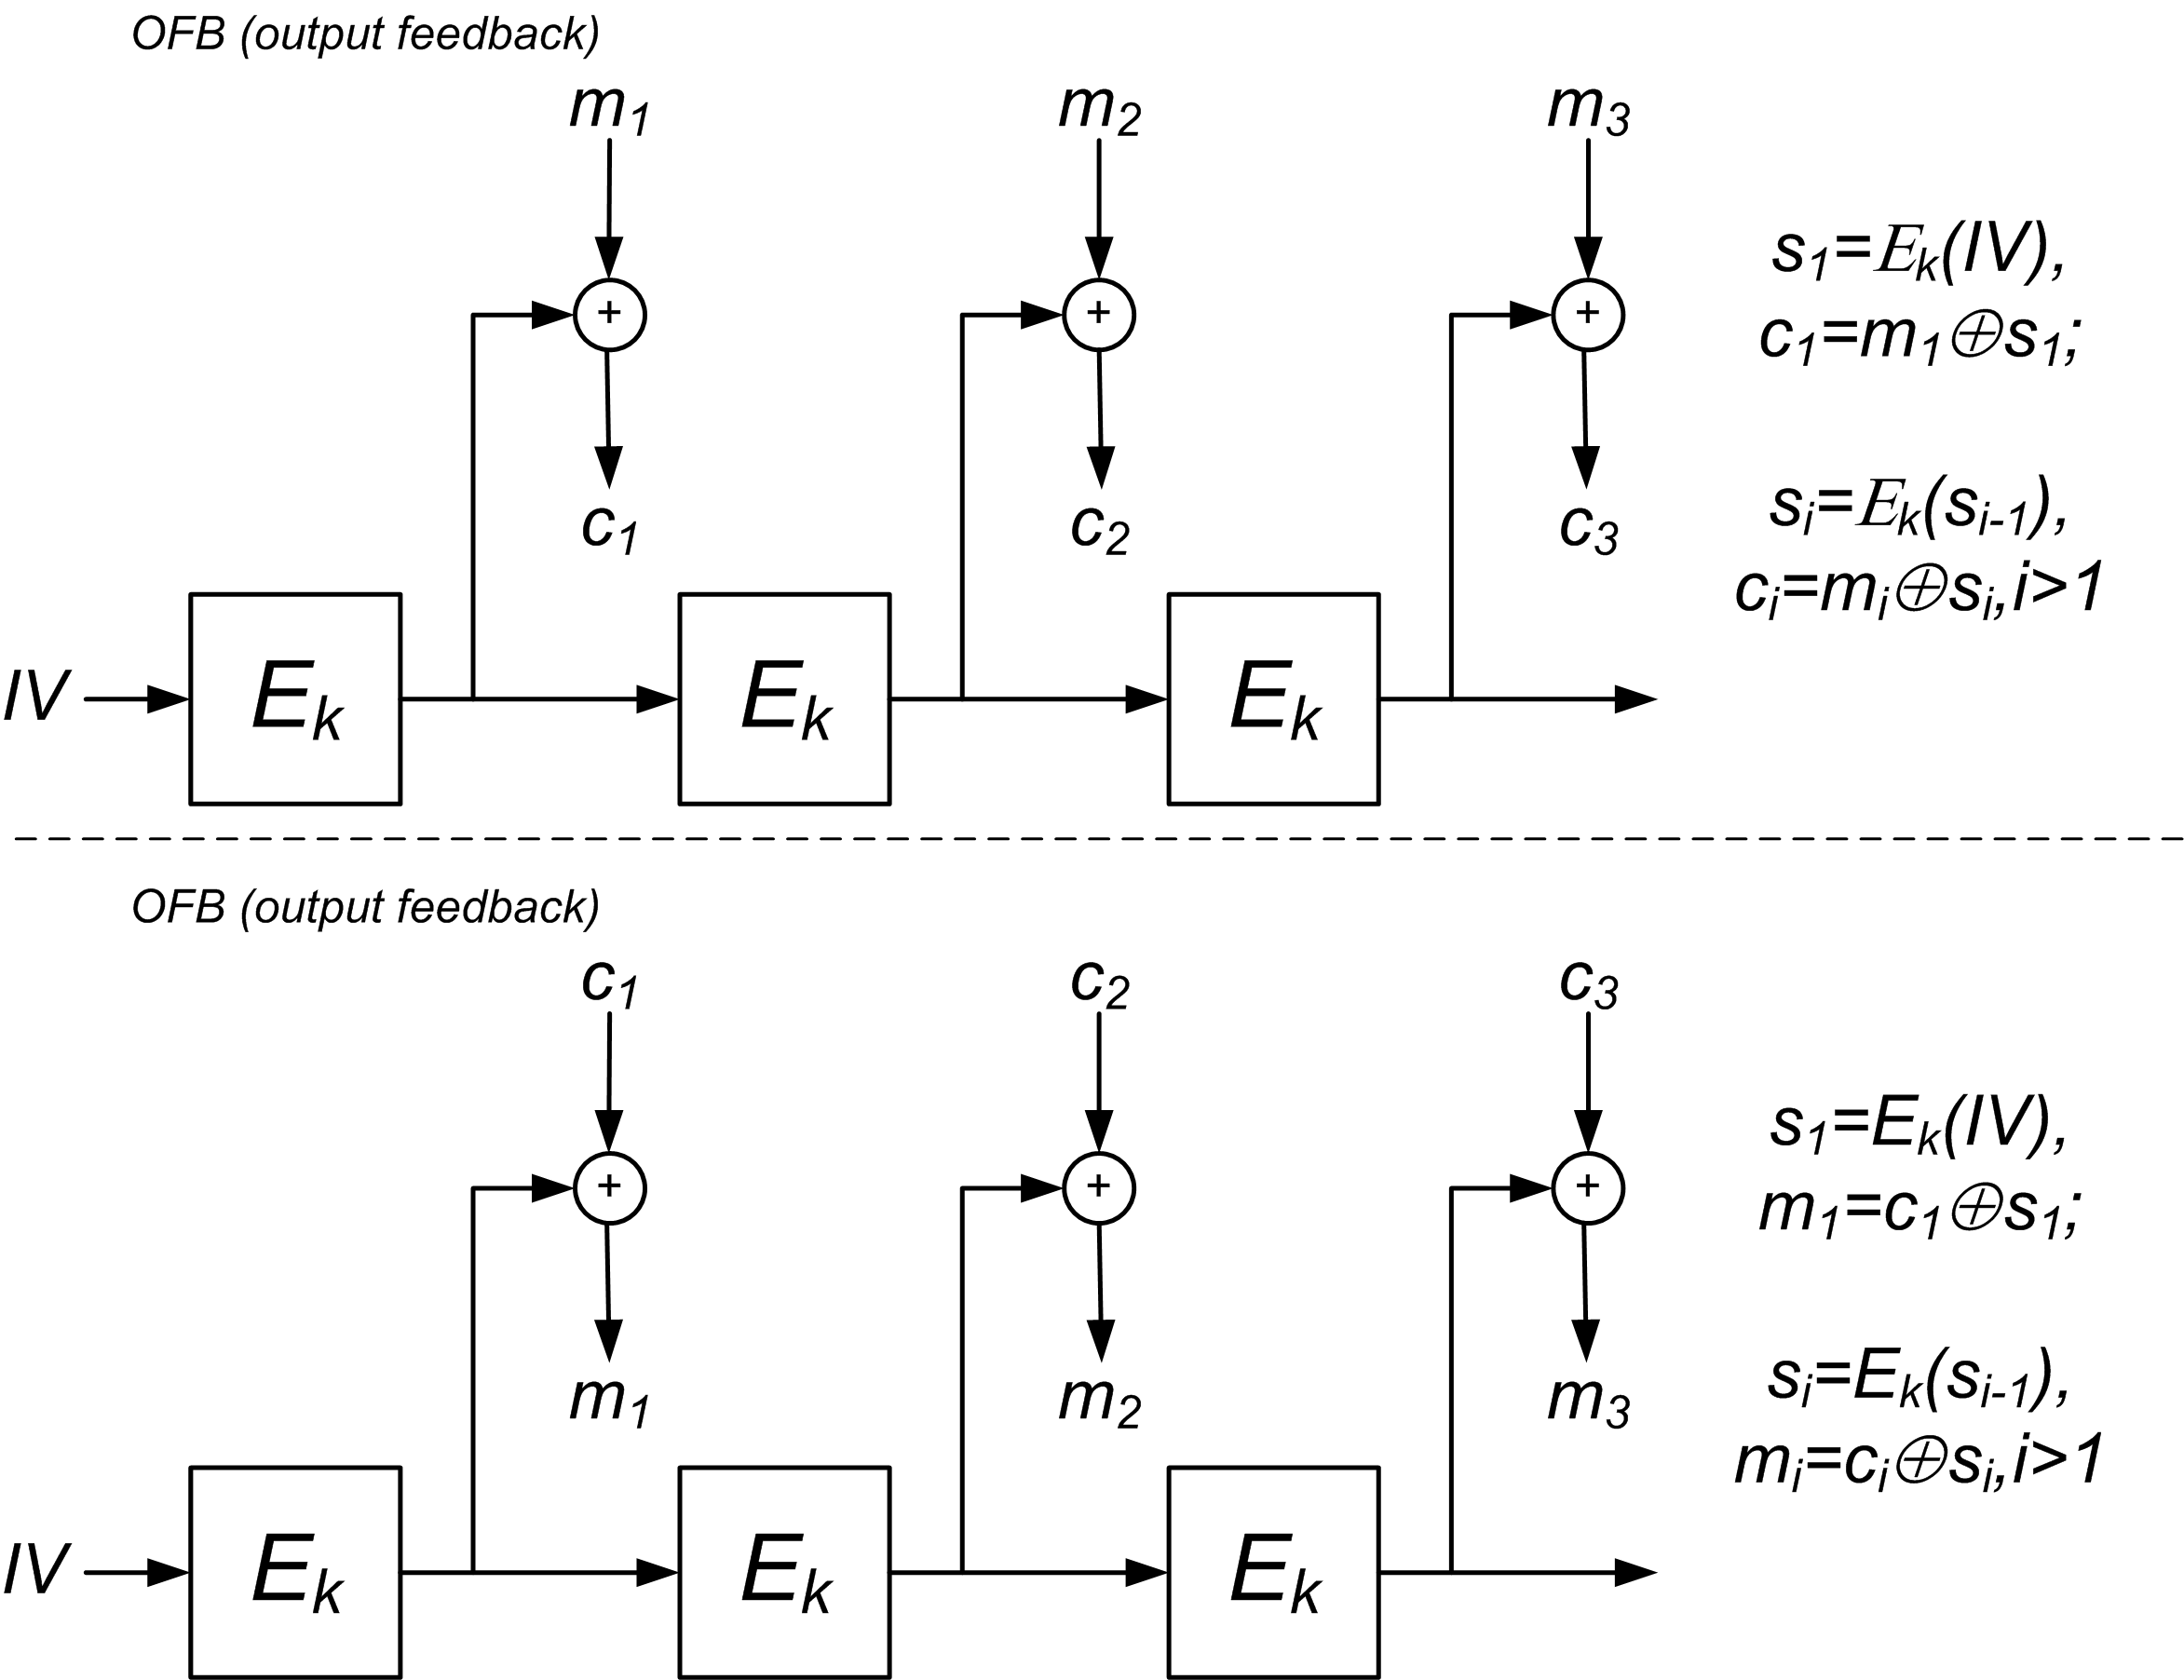
\includegraphics[width=.8\textwidth]{pict/ofb} 
                \caption{OFB}\label{pict:ofb}
            }
        \end{center}
    \end{figure} 
    \mode<article>{См. рисунок \ref{pict:ofb}}
\end{frame}


\begin{frame}
    \frametitle{CTR}
    
    \begin{figure}
        \begin{center}
            \mode<presentation>{ 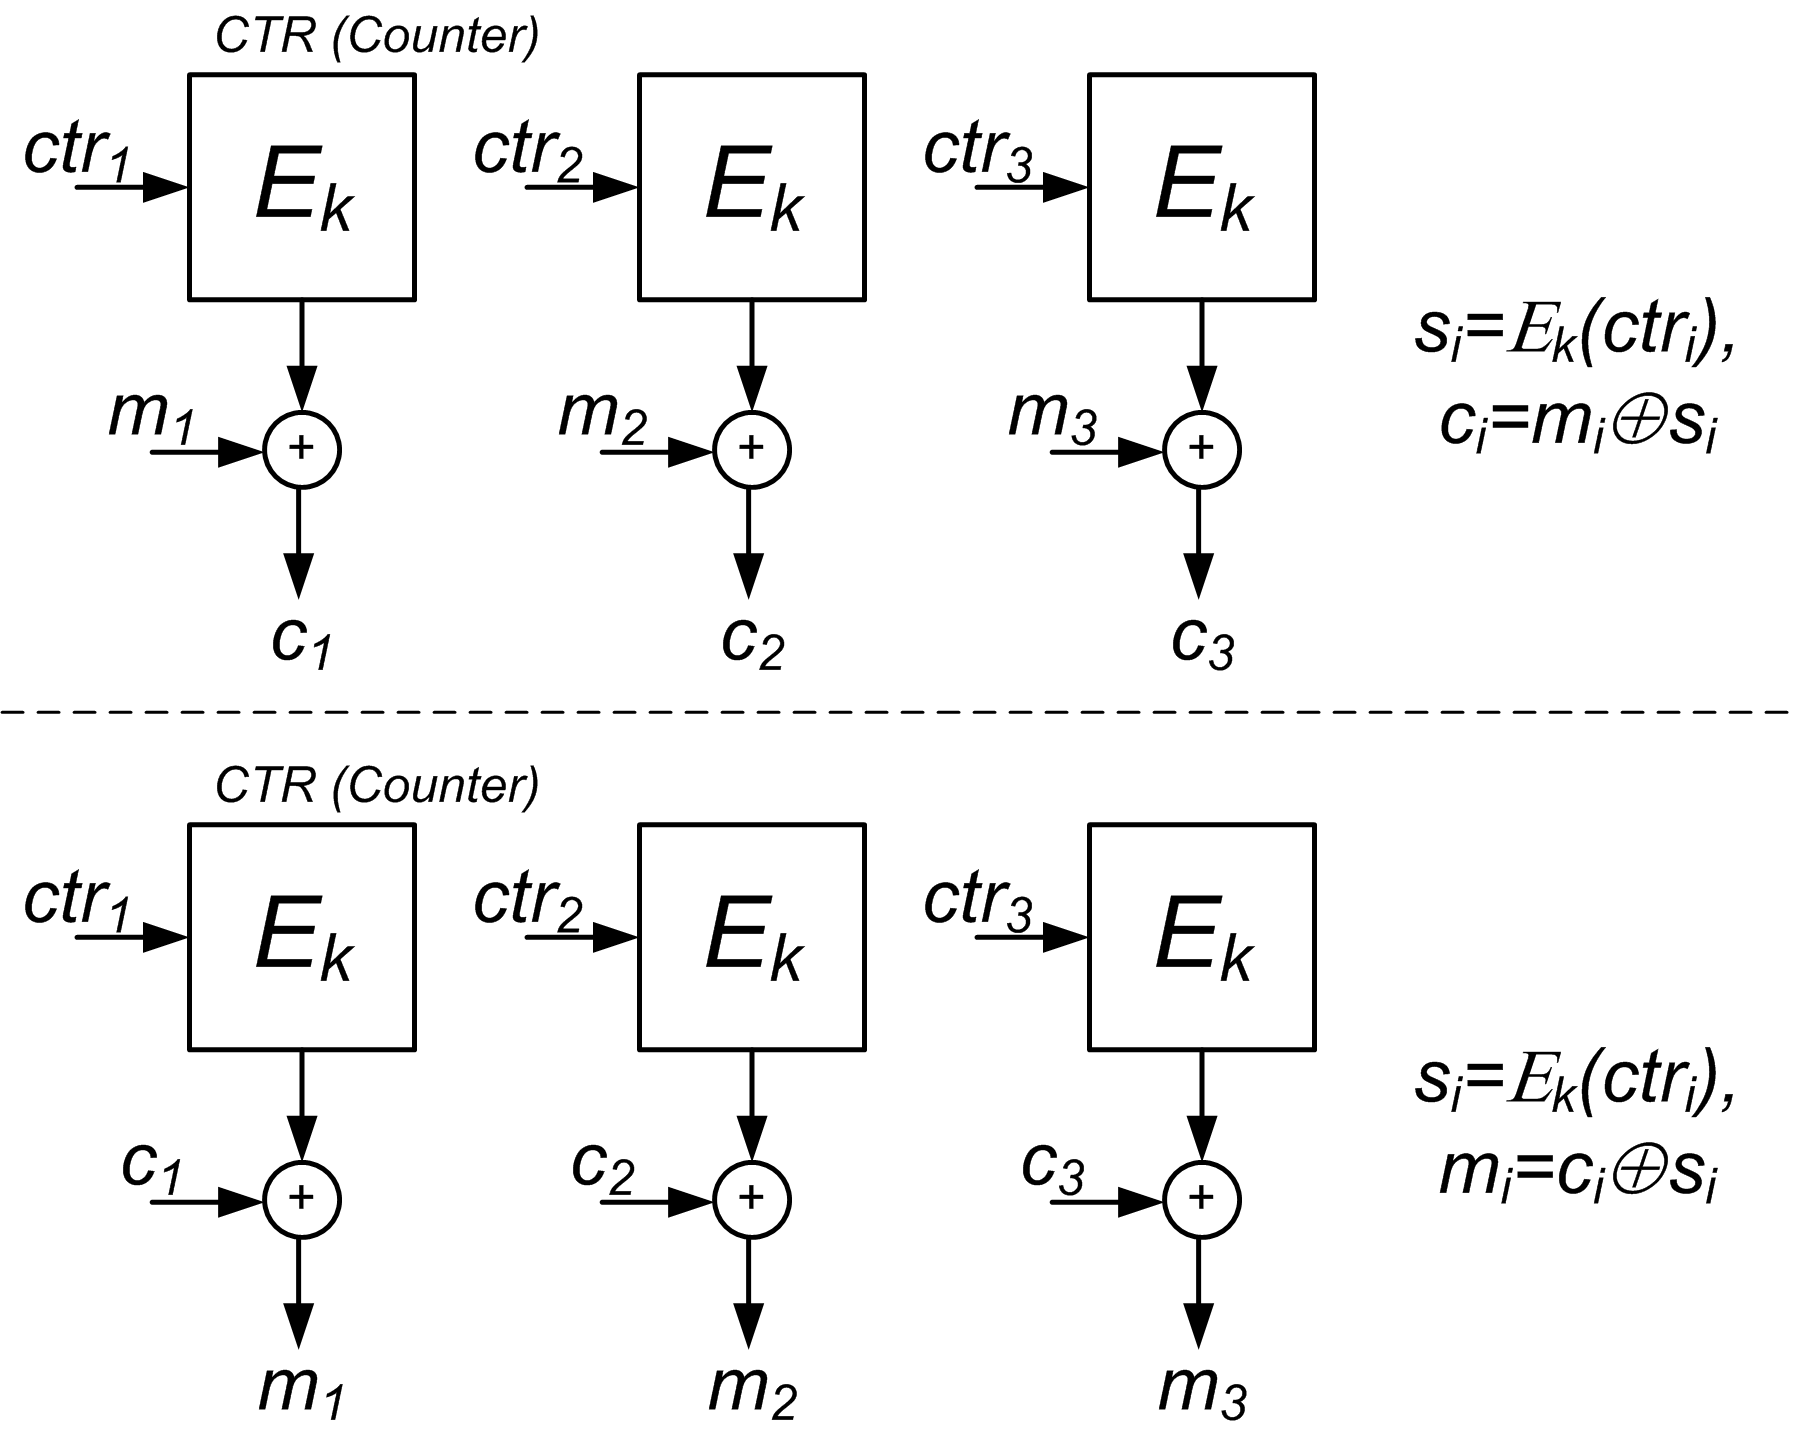
\includegraphics[height=.73\textheight]{pict/ctr} }
            \mode<article>{ 
                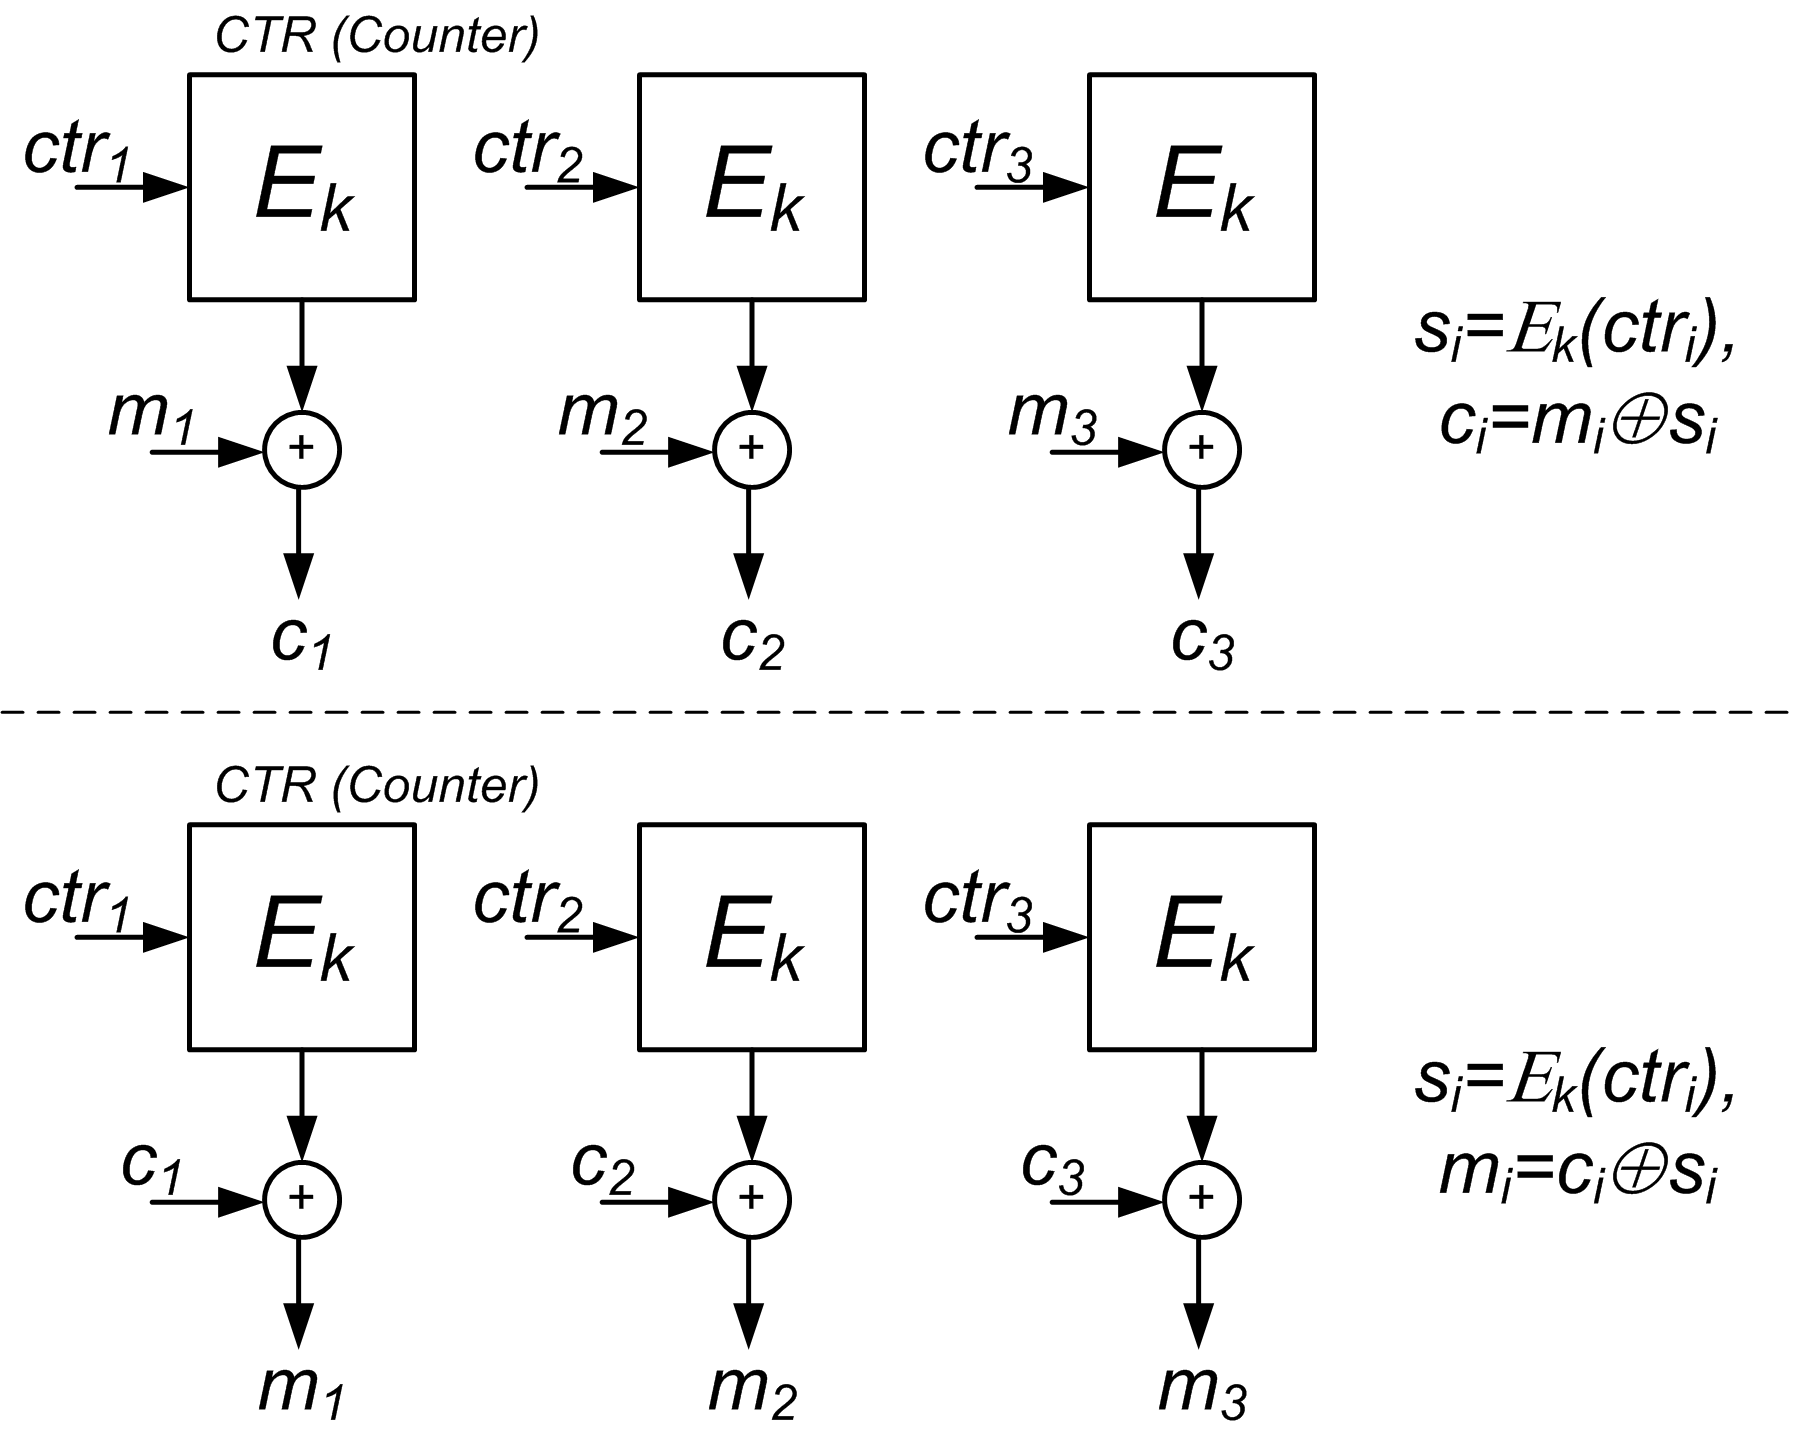
\includegraphics[width=.8\textwidth]{pict/ctr} 
                \caption{CTR}\label{pict:ctr}
            }
        \end{center}
    \end{figure} 
    \mode<article>{См. рисунок \ref{pict:ctr}}
\end{frame}


\section{Поточные шифры}


При шифровании больших объемов данных в реальном времени требуется очень быстрый шифр, и не каждый блочный шифр удовлетворяет таким требованиям. Поток ключей, основанных на основном ключе, обычно генерируется с помощью однозначно детерминированных алгоритмов.

\begin{frame}
    \frametitle{Представители симметричных поточных шифров}
    \framesubtitle{Stream ciphers}
    
    \begin{itemize}
        \item RC4
        \item HC-128 
        \item Grain v1
        \item Rabbit 
        \item MICKEY v2
        \item Salsa20/12 
        \item Trivium
        \item Sosemanuk
        \item и т.д\footnote{Все перечисленные, кроме первого --- лауреаты eStream}.
    \end{itemize} 
\end{frame}


\begin{frame}
    \frametitle{Типы симметричных поточных шифров}
    
    \begin{itemize}
        \item \alert{Синхронные}, в которых поток ключей формируется независимо от открытого текста или шифротекста\footnote{Примером может являться \alert{двоичный аддитивный поточный шифр}: биты ключа складываются с битами открытого текста по XOR.}.
        \item \alert{Асинхронные} (самосинхронизирующиеся), которые используют $N$ предыдущих бит потока шифротекста\footnote{Примером может являться \alert{блочный} шифр в режиме CFB}. 
    \end{itemize} 
\end{frame}


\subsection{РСЛОС (LFSR)}


\begin{frame}
    \frametitle{Регистр сдвига с обратной связью}
    \framesubtitle{FSR (Feedback Shift Register)}
    
    \begin{figure}
        \begin{center}
            \mode<presentation>{ 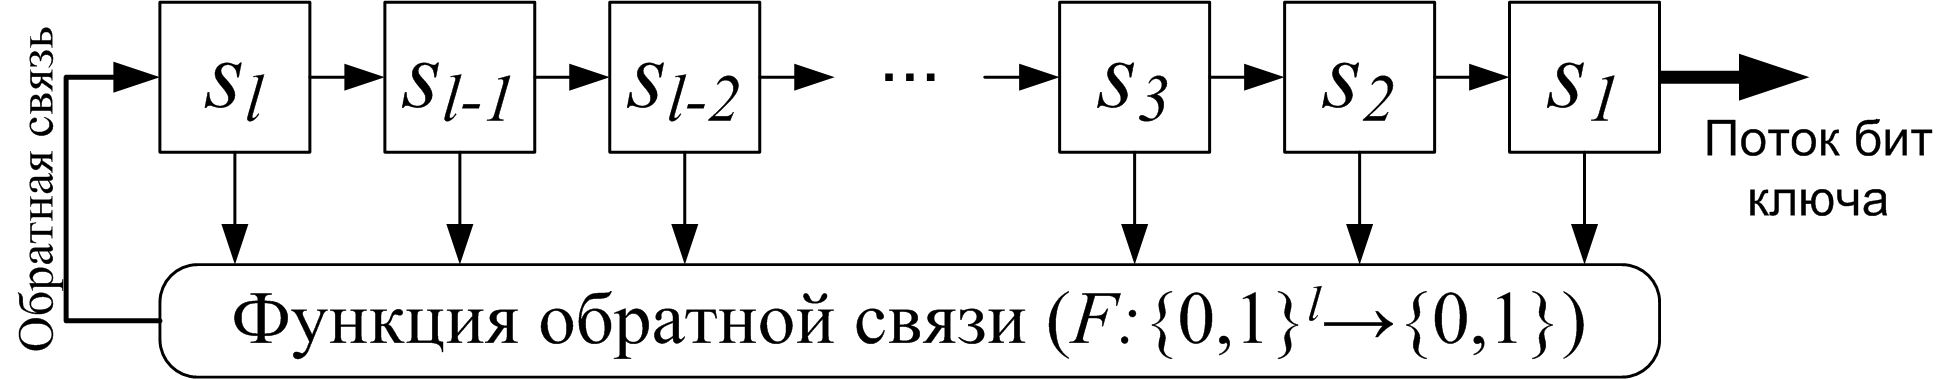
\includegraphics[width=.93\textwidth]{pict/fsr} }
            \mode<article>{ 
                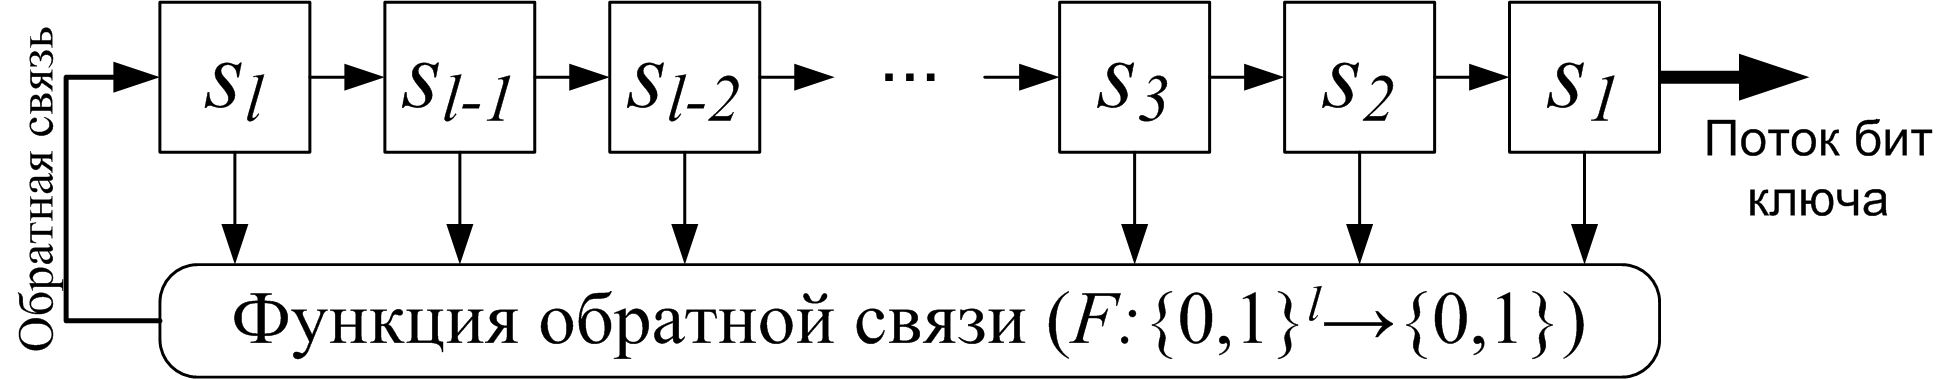
\includegraphics[width=.8\textwidth]{pict/fsr} 
                \caption{FSR}\label{pict:fsr}
            }
        \end{center}
    \end{figure} 
    \mode<article>{См. рисунок \ref{pict:fsr}}
\end{frame}


\begin{frame}
    \frametitle{РСЛОС. Регистр сдвига с \alert{линейной} обратной связью}
    \framesubtitle{LFSR (Linear Feedback Shift Register)}
    
    Когда нелинейная функция --- это XOR, FSR называется LFSR (РСЛОС).
    \begin{figure}
        \begin{center}
            \mode<presentation>{ 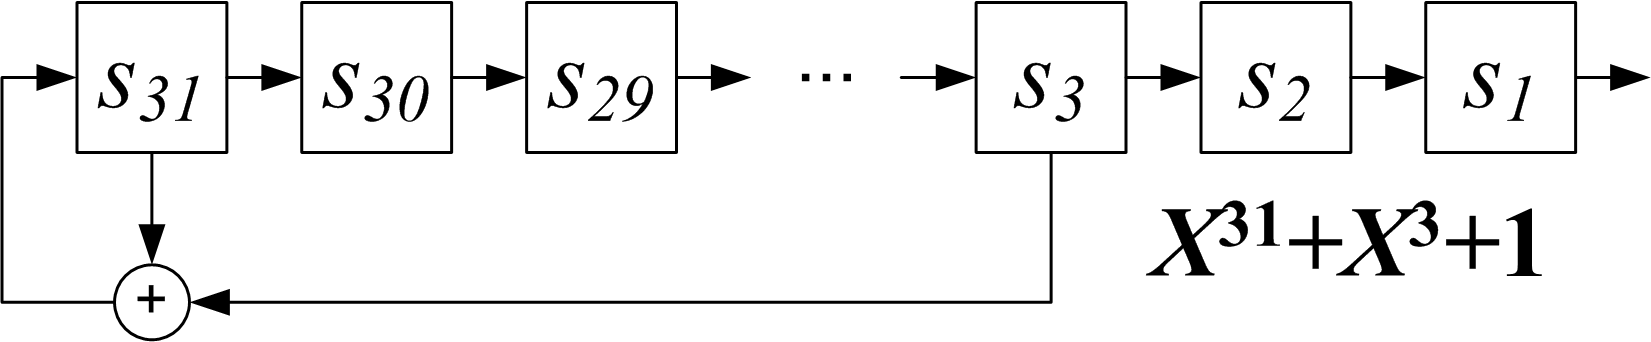
\includegraphics[width=.73\textwidth]{pict/lfsr} }
            \mode<article>{ 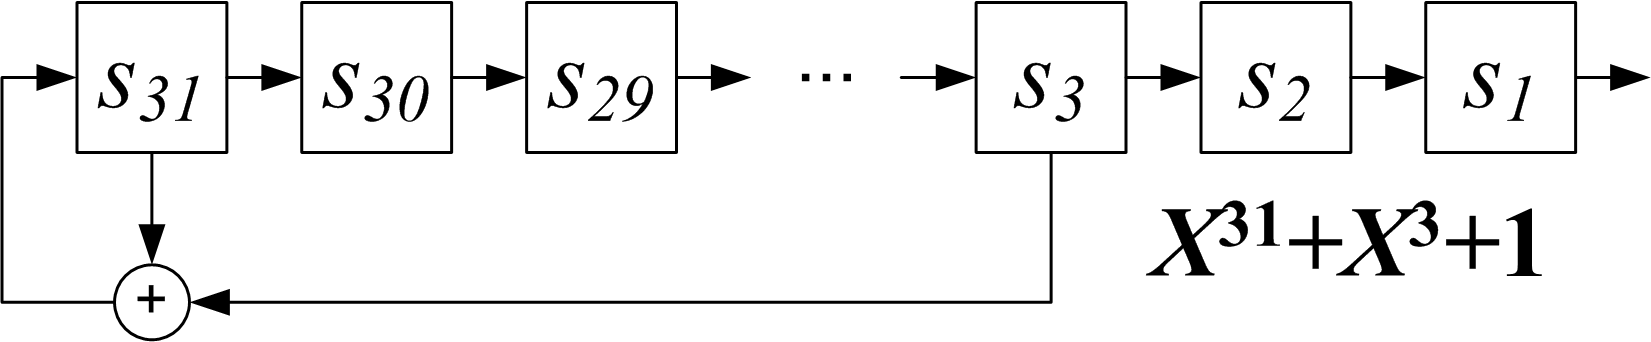
\includegraphics[width=.8\textwidth]{pict/lfsr} }
        \end{center}
        \caption{РСЛОС для полинома $X^{31}+X^3+1$}\label{pict:lfsr}
    \end{figure} 
    \mode<article>{См. рисунок \ref{pict:lfsr}}
    Каждый последующий бит $s_i$ потока $S=\{s_1,s_2,\ldots\}$ получается как
    \[s_i=c_1s_{i-1}\oplus c_2s_{i-2}\oplus\cdots\oplus c_ls_{i-l}=\bigoplus_{j=1}^{l}c_js_{i-j},\]
    где $i>l$, а $c_i$ соответсвует отводу.
\end{frame}


\begin{frame}
    \frametitle{РСЛОС. Регистр сдвига с \alert{линейной} обратной связью}
    
    Каждому РСЛОС можно поставить в соответствие полином:
    \[g(X)=1+c_1X+c_2X^2+\cdots+c_lX^l.\]
    Период последовательности ключей $S$ будет равен максимально возможному $2^l-1$, если полином $g(X)$ \alert{примитивен}.
    
    \begin{block}{Шифрование/расшифрование}
    Ячейки РСЛОС инициализируются битами ключа $\{s_ls_{l-1}\cdots s_1\}=K$ и далее каждый $i$-й бит открытого текста складывается по XOR с битом на выходе регистра после $i$-го сдвига: $C_i=M_i\oplus\text{РСЛОС}_1^i$. Расшифрование также элементарно: $M_i=C_i\oplus\text{РСЛОС}_1^i$.
    \end{block}
\end{frame}


\begin{frame}
    \frametitle{РСЛОС. Регистр сдвига с \alert{линейной} обратной связью}

    Основным недостатком РСЛОС является его линейность, так, если злоумышленник получит $2l$ бит ключевого потока он воостановит конфигурацию регистра и сможет воспроизводить поток. Поэтому обычно используют $n$ регистров разной конфигурации, выходы которых комбинируются нелинейной булевой функцией\footnote{Например: $f(x_1,x_2,x_3,x_4,x_5)=1\oplus x_2\oplus x_3 \oplus x_4x_5 \oplus x_1x_2x_3x_5$}.
    \begin{figure}
        \begin{center}
            \mode<presentation>{ 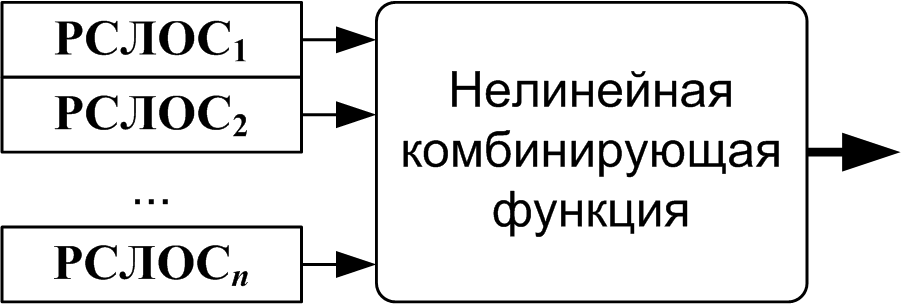
\includegraphics[width=.63\textwidth]{pict/lfsrMix} }
            \mode<article>{ 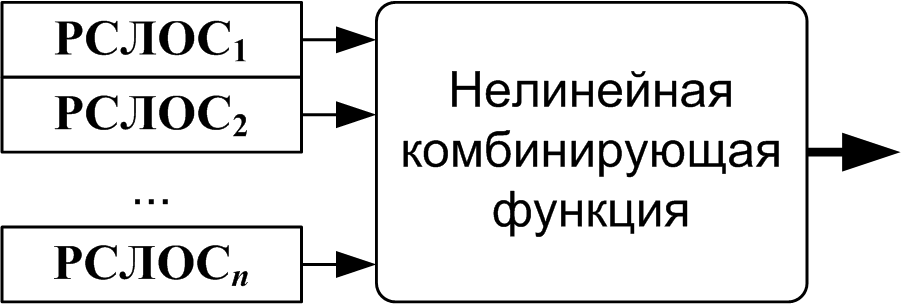
\includegraphics[width=.8\textwidth]{pict/lfsrMix} }
        \end{center}
        \caption{Комбинирование РСЛОС}\label{pict:lfsrMix}
    \end{figure} 
    \mode<article>{См. рисунок \ref{pict:lfsrMix}}
\end{frame}


\subsection{RС4}


Генерирует не последовательность бит, а последовательность байт, что, согласитесь, удобнее для программной реализации. Используется в протоколах WEP, SSL, для шифрования потоковых аудио/видео-данных. Созданный в 1987 году, был ноу-хау компании RSAsecurity, но в 1994 году произошла утечка кода.

В основе шифра лежит 256 байтный массив S, содержащий соответственно все значения от 0 до 255 (т.е. все комбинации 8-и бит). Каждый следующий байт генерируемой последовательности выбирается из этого массива. Шифр синхронный. Вначале упорядоченные по возрастанию элементы S подвергается перестановке, зависящей от ключа. Эта процедура \verb"rc4_init" инициализирует генератор. Получавшийся в результате массив S полностью определяет последовательность, которая будет сгенерирована.

\begin{frame}[fragile]
    \frametitle{RC4}

    \begin{definition}
        RC4 --- Rivest Cipher 4 (Ron’s Code)\footnote{RC4 создан Роном Райвестом (Ron Rivest) во время его работы в  RSA Security в 1987 году}
    \end{definition}

Состояние RC4-генератора определяют следующие данные:
\begin{semiverbatim}
    unsigned char S[256]; 
    unsigned int i, j;
\end{semiverbatim}
\end{frame}


\begin{frame}[fragile]
    \frametitle{RC4}
    \framesubtitle{Инициализация}

Генератор должен быть проинициализирован ключом \verb"key" \footnote{Массив байт длиной \verb"keyLen"} на <<холостом ходу>>:
\begin{semiverbatim}
\uncover<1->{\alert<1->{void rc4_init(unsigned char *key, unsigned int keyLen) \{  }}
\uncover<2->{\alert<2>{    for (i = 0; i < 256; i++) \{ }}
\uncover<2->{\alert<2>{        S[i] = i; }}
\uncover<2->{\alert<2>{    \} }}
\uncover<3->{\alert<3>{    for (i = j = 0; i < 256; i++) \{ }}
\uncover<3->{\alert<3>{        j = (j + key[i \% keyLen] + S[i])&255; }}
\uncover<3->{\alert<3>{        swap(&S[i], &S[j]); }}
\uncover<3->{\alert<3>{    \} }}
\uncover<4->{\alert<4>{    i = j = 0; }}\uncover<5->{}
\uncover<1->{\alert<1->{\} }}
\end{semiverbatim}
\end{frame}


\begin{frame}[fragile]
    \frametitle{RC4}
    \framesubtitle{Генерация байт ключа}

Каждый сгенерированный функцией \verb"rc4_output" байт складывается по XOR с соответствующим байтом открытого текста.
\begin{semiverbatim}
\uncover<1->{\alert<1->{unsigned char rc4_output() \{  }}
\uncover<2->{\alert<2>{    i = (i + 1)&255;  }}
\uncover<2->{\alert<2>{    j = (j + S[i])&255;  }}
\uncover<3->{\alert<3>{    swap(&S[i], &S[j]);  }}
\uncover<4->{\alert<4>{    return S[ (S[i] + S[j])&255 ];  }}\uncover<5->{}
\uncover<1->{\alert<1->{\}  }}
\end{semiverbatim}
\end{frame}

\appendix


\begin{frame}
\frametitle{Источники и полезные ссылки}
    \begin{enumerate}
        \item Режимы работы блочного шифра \cite{bib:mao:modernCrypto,bib:smart:crypto}. 
        \item Поточные шифры \cite{bib:smart:crypto,bib:chmora:crypto}. 
        \item Классика жанра: \cite{bib:shneir:applCrypto}. 
        \item История конкурса на стандарт среди поточных шифров: \cite{bib:misc:estream}.
    \end{enumerate}    
\end{frame}


\begin{frame}[allowframebreaks]{Библиография}
    \bibliographystyle{gost780u}
    \bibliography{./../bibliobase}
\end{frame}

\end{document}